
\chapter{Results}

The following results are exploratory in nature, and After some poor initial results the focus was laid on proving that
the network can perform at all, rather than fine-tuning hyperparameters towards optimal performance. This decision was
in part motivated by a prioritization of gaining neuroscientific insights over achieving minimal test loss. It should be
noted, that training the network is computationally quite costly (c.f. Section \ref{sec-benchmark}) which turned
parameter studies into a time-consuming process.

Early experiments showed that the network is rather sensitive to parameter changes. The search for default parameters
took some effort, as a certain heterogeneity exists in the two existing implementations
\citep{sacramento2018dendritic,Haider2021}, both in hyperparameters as in the simulation environment. This model
includes properties of both variants, while relying more strongly on the LE implementation. Unless stated otherwise,
neurons employ prospective activation functions in all simulations. So far, no drawbacks to this mechanism have
presented themselves, and learning speed can be increased drastically compared to the original implementation. The full
default parametrization is shown in Supplementary Table \ref{tab-params}. Since it was anticipated that the spiking
implementation would perform worse than the rate-based variant, the first goal was to measure how big this difference in
performance is. Furthermore, a relevant question was to what degree the synaptic delays enforced by NEST would influence
performance of the rate model. These questions will be answered in the upcoming sections. Note that not all experimental
results were given their own Figures. In these cases, plots can be found in the electronic supplementary material.


\section{The self-predicting state}

As a first comparison between the three implementations, the pre-training towards a self-predicting state (cf.
\citep{sacramento2018dendritic}[Fig. S1]) was performed. For this experiment, no target signal is provided at the output
layer, and the network is tasked with learning to self-predict top-down input. The network is initialized with fully
random weights and stimulated with random inputs from a uniform distribution between 0 and 1. A comparison of the four
error metrics between implementations is shown in Fig. \ref{fig-self-pred}.



\begin{figure}[h]
    \centering
    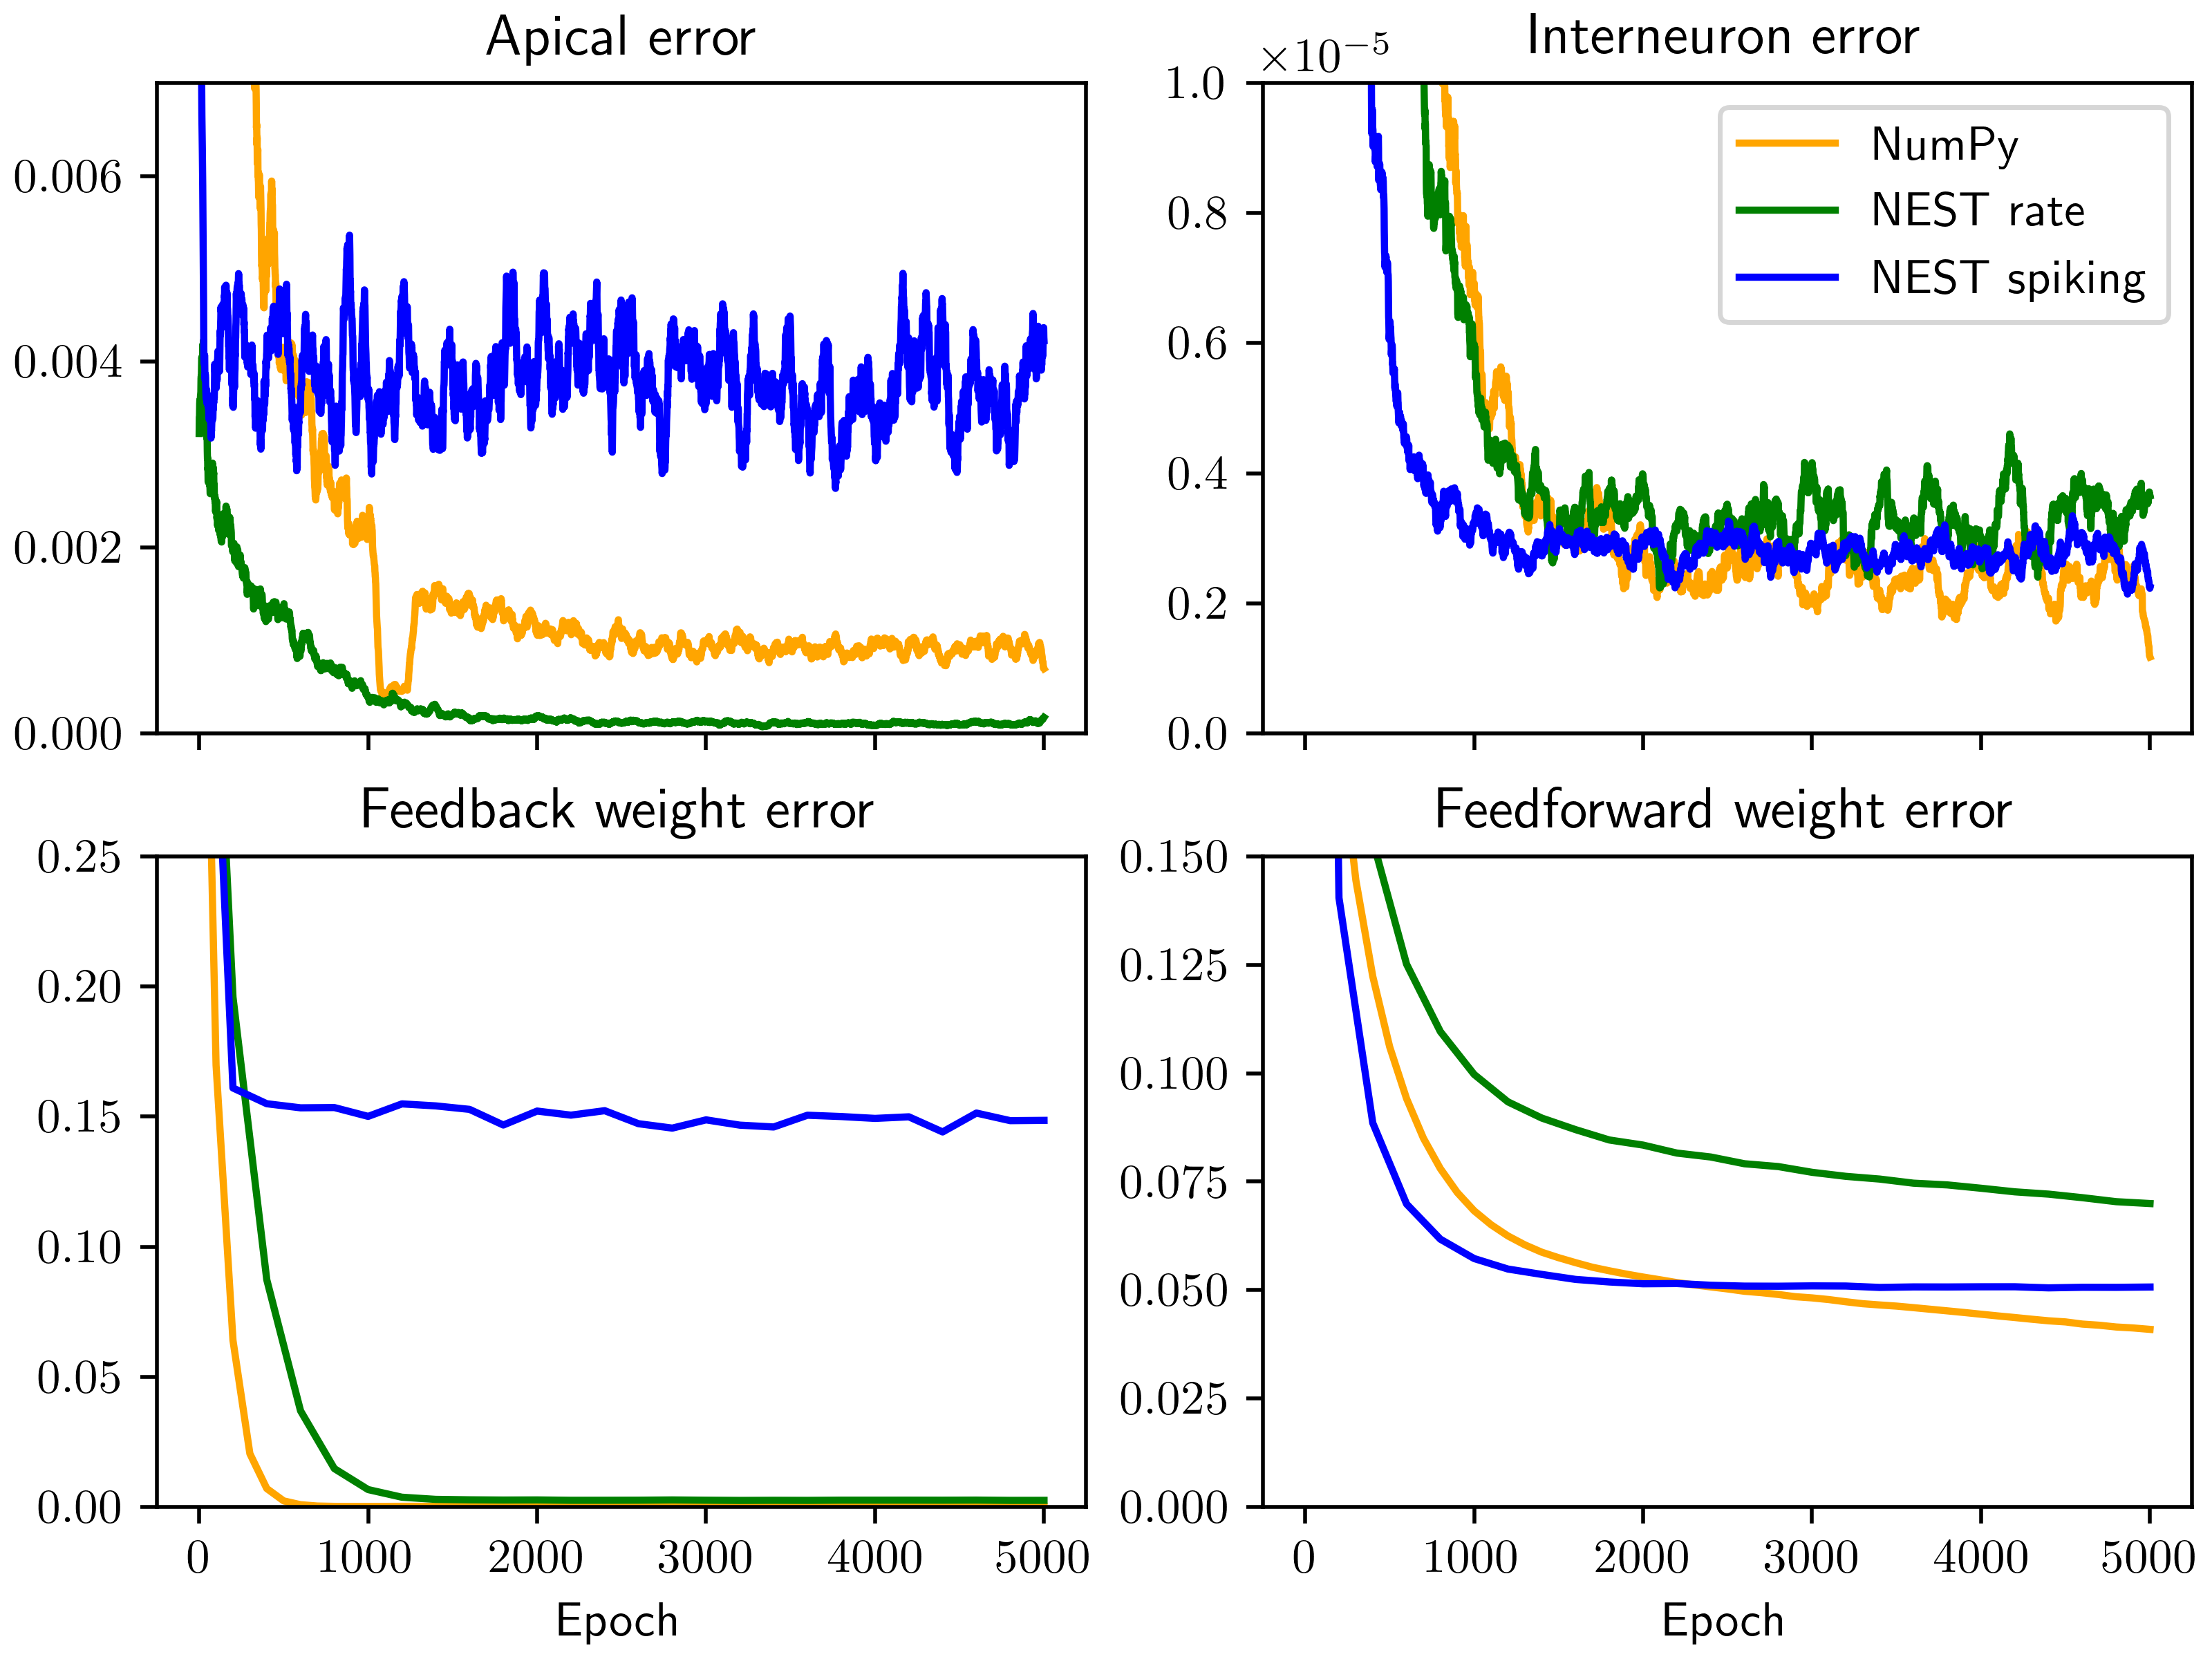
\includegraphics[width=0.9\textwidth]{fig_self_prediction}
    \caption[Training towards the self-predicting state]{Training towards the self-predicting state. All implementations
        learn to predict self-generated top-down signals. Networks were initialized with the same random weights for
        dimensions $[5, 8, 3]$, and stimulated with $5000$ samples of random input for $100ms$ each. As described in
        \citep{sacramento2018dendritic}, during this phase only $Pyr \rightarrow Intn$ and $Intn \rightarrow Pyr$
        weights are plastic ($\eta^{pi}=0.05, \eta^{ip}=0.02375, \eta^{up}_0=\eta^{up}_1=\eta^{down}=0$).}
    \label{fig-self-pred}
\end{figure}

Both rate neuron implementations were able to reach comparable values for all error metrics after roughly the same time.
The exact values that errors converge on differs slightly between implementations, with no implementation being clearly
superior. This is an important result for upcoming experiments, as it indicates that both training environment (current
injections, simulation time, membrane reset, readouts, etc.) and the actual neuron model of the NEST version adequately
replicate the original model.

For the spiking variant, interneuron- and its corresponding feedfworward weight error are comparable to the other
implementations. In fact these metrics appear to converge slightly faster to comparable values. The primary limitation
of this version are the apical error and the closely correlated FB error. After appearing to converge very quickly, the
two metrics stagnate at very high levels. These high errors correlate with strong fluctuations of the apical
compartment. These fluctuations can likely at least in part be attributed to low spike frequencies. This was confirmed
by repeating the experiment with $\psi=1500$, which alleviated the issue to a degree (results not shown). Yet, error
values were still inferior to the rate models, and this change came at the cost of substantially increased training
time. Therefore, this approach was not pursued much further. A different possible solution is, to increase the membrane
capacitance of the apical compartment in order to smooth out the fluctuations induced by individual spikes. This will be
discussed in Section \ref{sec-c-m-api}.

In most simulations in the literature, the network is initialized to an ideal self-predicting state. Furthermore,
feedback weights are non-plastic in many experiments ($\eta^{pi}=\eta^{down}=0$). Therefore, a failure to perfectly
learn this weight symmetry should not fundamentally hinder learning. For the time being, showing that the network
approaches a self-predicting state was deemed a sufficient result.


\section{Presentation times and latent Equilibrium}\label{sec-le-tpres}

In order to validate the performance of the NEST implementations on a learning task, the parameter study from
\citep{Haider2021}[Fig. 3] was replicated. In this experiment, the network is trained with different stimulus
presentation times $t_{pres} \in \{0.3,\ 500\}ms$. Performance of the original Dendritic error network is compared to
the improved model which employs LE. Due to the costly computation of the network under such long $t_{pres}$, a simple
artificial classification dataset was used. The \textit{Bars-dataset} is defined for $3\times3$ input- and $3$ output
neurons. It consists of three horizontal, three vertical, and two diagonal bars in the $3\times3$ grid, which are to be
encoded in a 'one-hot-vector' at the output layer. In the experiment, networks of $9-30-3$ pyramidal neurons per layer
were trained for 1000 Epochs of 24 samples each. Networks were initialized to the self-predicting state and only
feedforward $Pyr\rightarrow Pyr$ and $Pyr \rightarrow Intn$ synapses were plastic. Learning rates scaled inversely with
presentation times: $\eta^{ip}_0 = \frac{0.2}{t_{pres}}, \eta^{up}_0 = \frac{0.5}{t_{pres}}, \eta^{up}_1 =
    \frac{0.1}{t_{pres}}$. The results for the spiking NEST network are shown in Fig. \ref{fig-bars-le-snest}, while the
results for NumPy and Rate NEST variants are depicted in Supplementary Figures \ref{fig-bars-le-numpy} and
\ref{fig-bars-le-rnest}, respectively.


\begin{figure}[h]
    \centering
    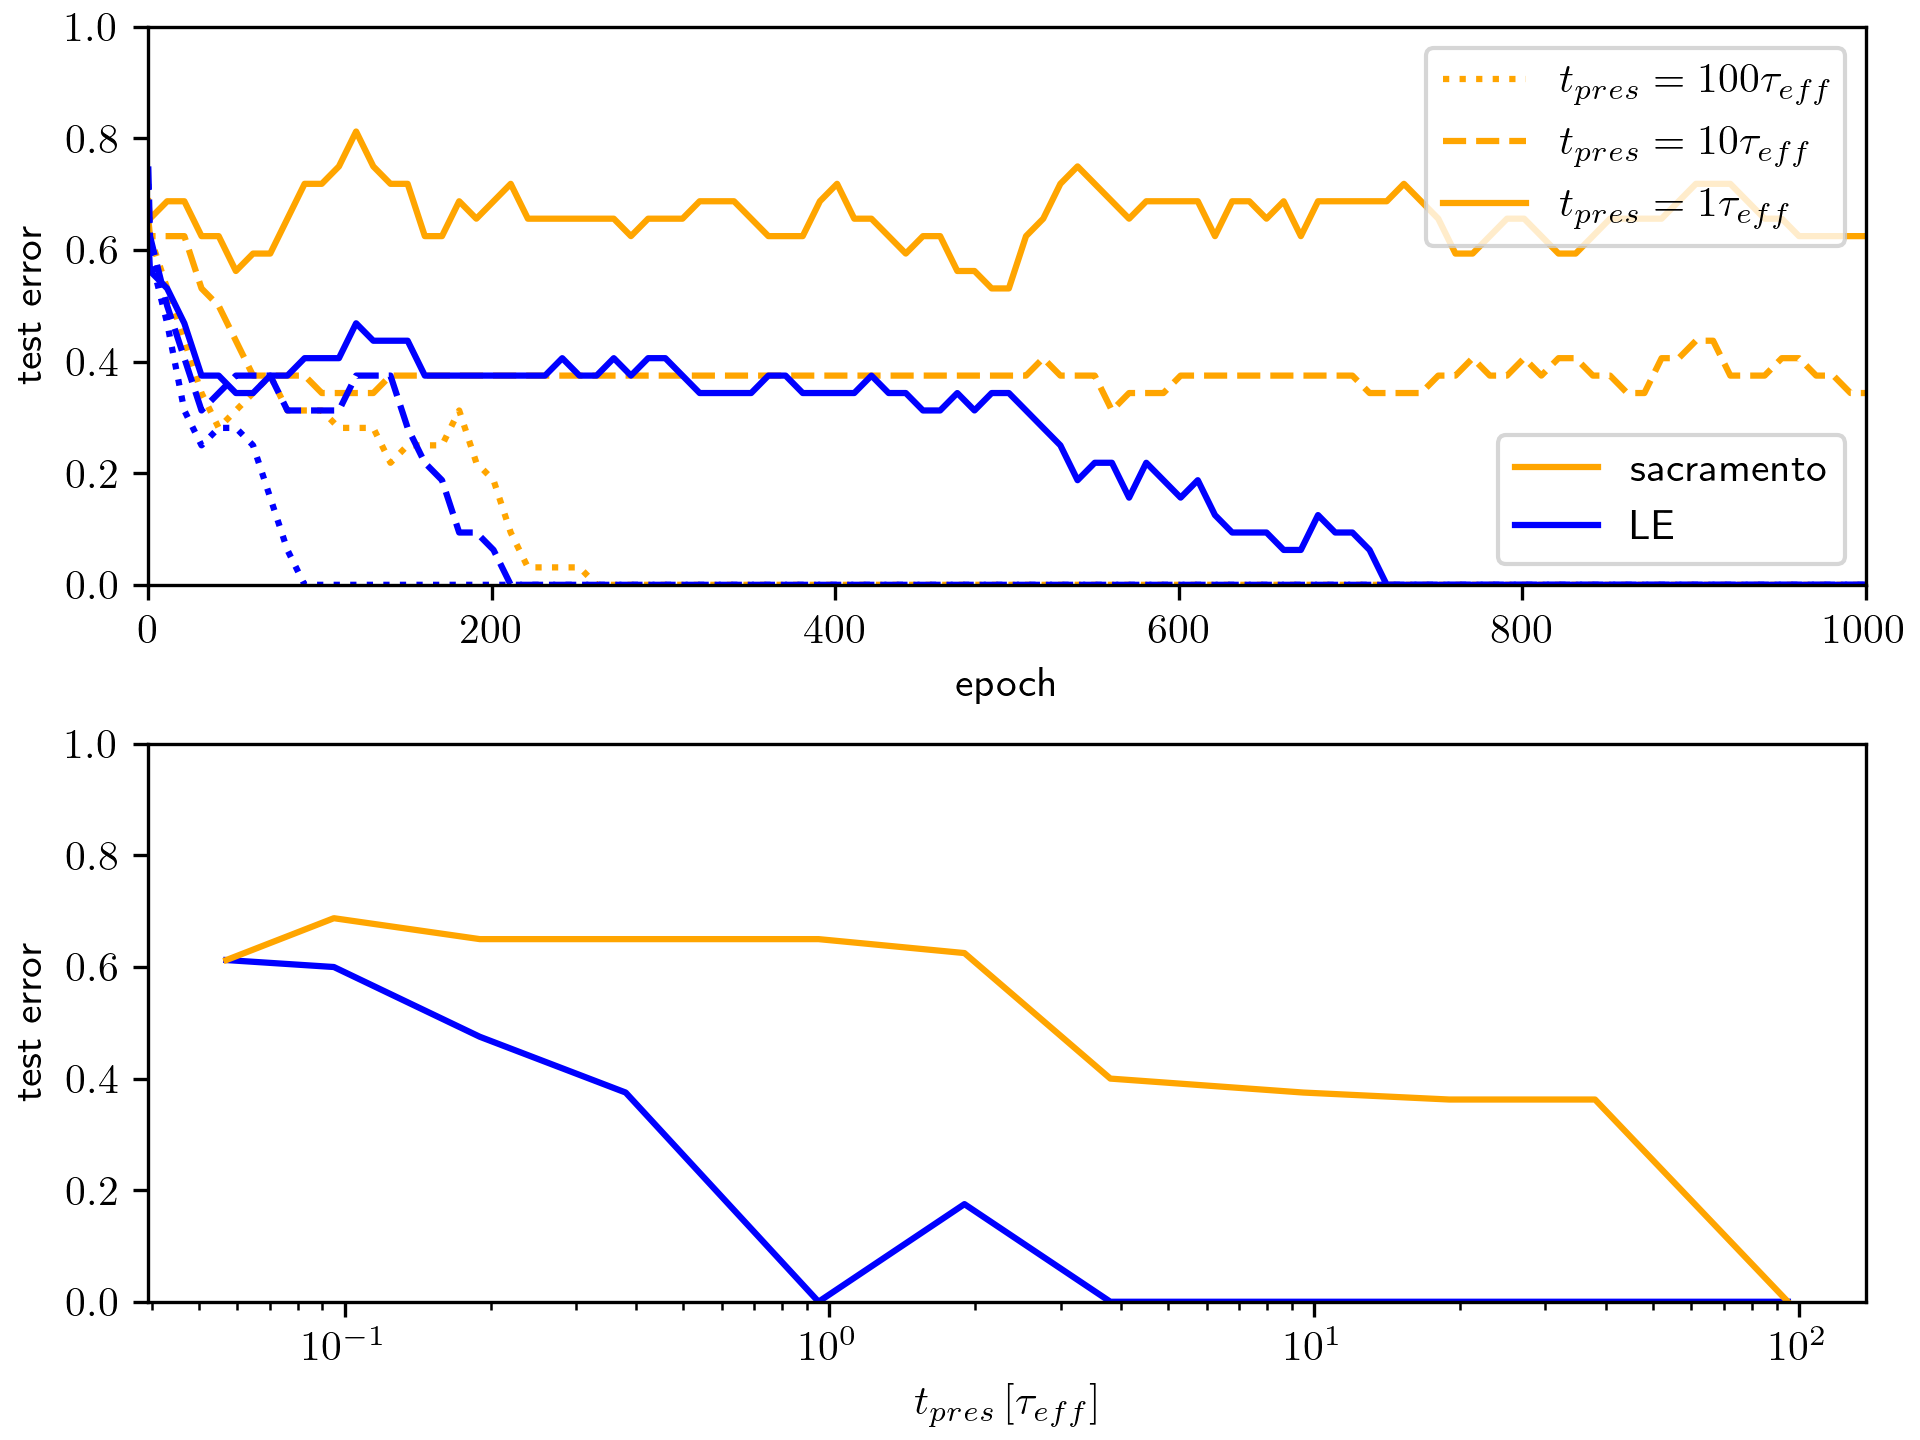
\includegraphics[width=0.9\textwidth]{fig_3_snest}
    \caption[Replication of Fig. 3 from \citep{Haider2021}.]{Replication of Fig. 3 from \citep{Haider2021} using
        networks of spiking neurons in the NEST simulator. \textbf{A:} Comparison between Original dendritic error
        network by and an identical network employing Latent Equilibrium. Shown is the training of networks with 9-30-3
        neurons on the Bars-dataset from with three different stimulus presentation times. \textbf{B:} Test performance
        after 1000 Epochs as a function of stimulus presentation time.}
    \label{fig-bars-le-snest}
\end{figure}

For the original dendritic error model, performance in all three implementations is close to being identical. This is an
important finding as it answers two open questions: Changes made for a NEST-compatible implementation were adequate and
result in identical learning between the rate-based implementations. Learning performance of the spiking model is
competitive, confirming the hypothesis that the spike-based dendritic plasticity model is capable of more complex credit
assignment tasks than previously shown. In this regard, the implementation can be considered a success.

The results for the LE network experiments are somewhat more interesting. For very long $t_{pres}$, both rate
implementations behave the same. Yet the NEST implementation requires considerably more epochs for training, as
$t_{pres}$ is reduced. For very low presentation times, this behavior was somewhat expected, due to the synaptic delay
enforced by NEST. The NumPy variant computes a full forward pass of the network during a single simulation step, as all
layers are processed in sequence. Only feedback signals from pyramidal neurons are delayed by one timestep in this
simulation backend. In NEST, all connections have a minimum synaptic delay of $\Delta t$. Therefore, for very short
presentation times the NEST network can not be expected to perform well, as signals have no time to traverse the
network. It remains an open question whether this feature alone explains the gradual decrease in performance observed
here, or if there is an undiscovered error within the novel neuron models or simulation environment. The exceptionally
short stimulus presentation times investigated by \citep{Haider2021} are themselves questionable in terms of biological
plausibility, as they are much lower than pyramidal neuron time constants \citep{McCormick1985}. Thus, no attempts were
made to improve performance for very low $t_{pres}$.

The spiking variant proved similarly sensitive to presentation times as the other NEST variant. While obtaining similar
final accuracy, it required - at best - twice as many stimulus presentations as its direct competitor. This result,
while somewhat expected, shows that for low $t_{pres}$, spiking communication leads to worse learning performance. It
also shows that the relaxation problem affects all communication schemes equally. While the utility of LE is
substantially higher for rate neurons, it does improve performance and efficiency of the spiking variant. For this
reason, LE will be turned on in all upcoming simulations.

\section{Approximating arbitrary functions}\label{sec-func-approx}

To confirm that the spiking network is capable of learning more complex tasks, it was trained to match the input-output
mapping of a separate teacher network. This is an established method for showing that a network can approximate
arbitrary functions. A performance comparison of several networks with different numbers of neurons in their hidden
layers is depicted in Fig. \ref{fig-func-approx}.


\begin{figure}[h]
    \centering
    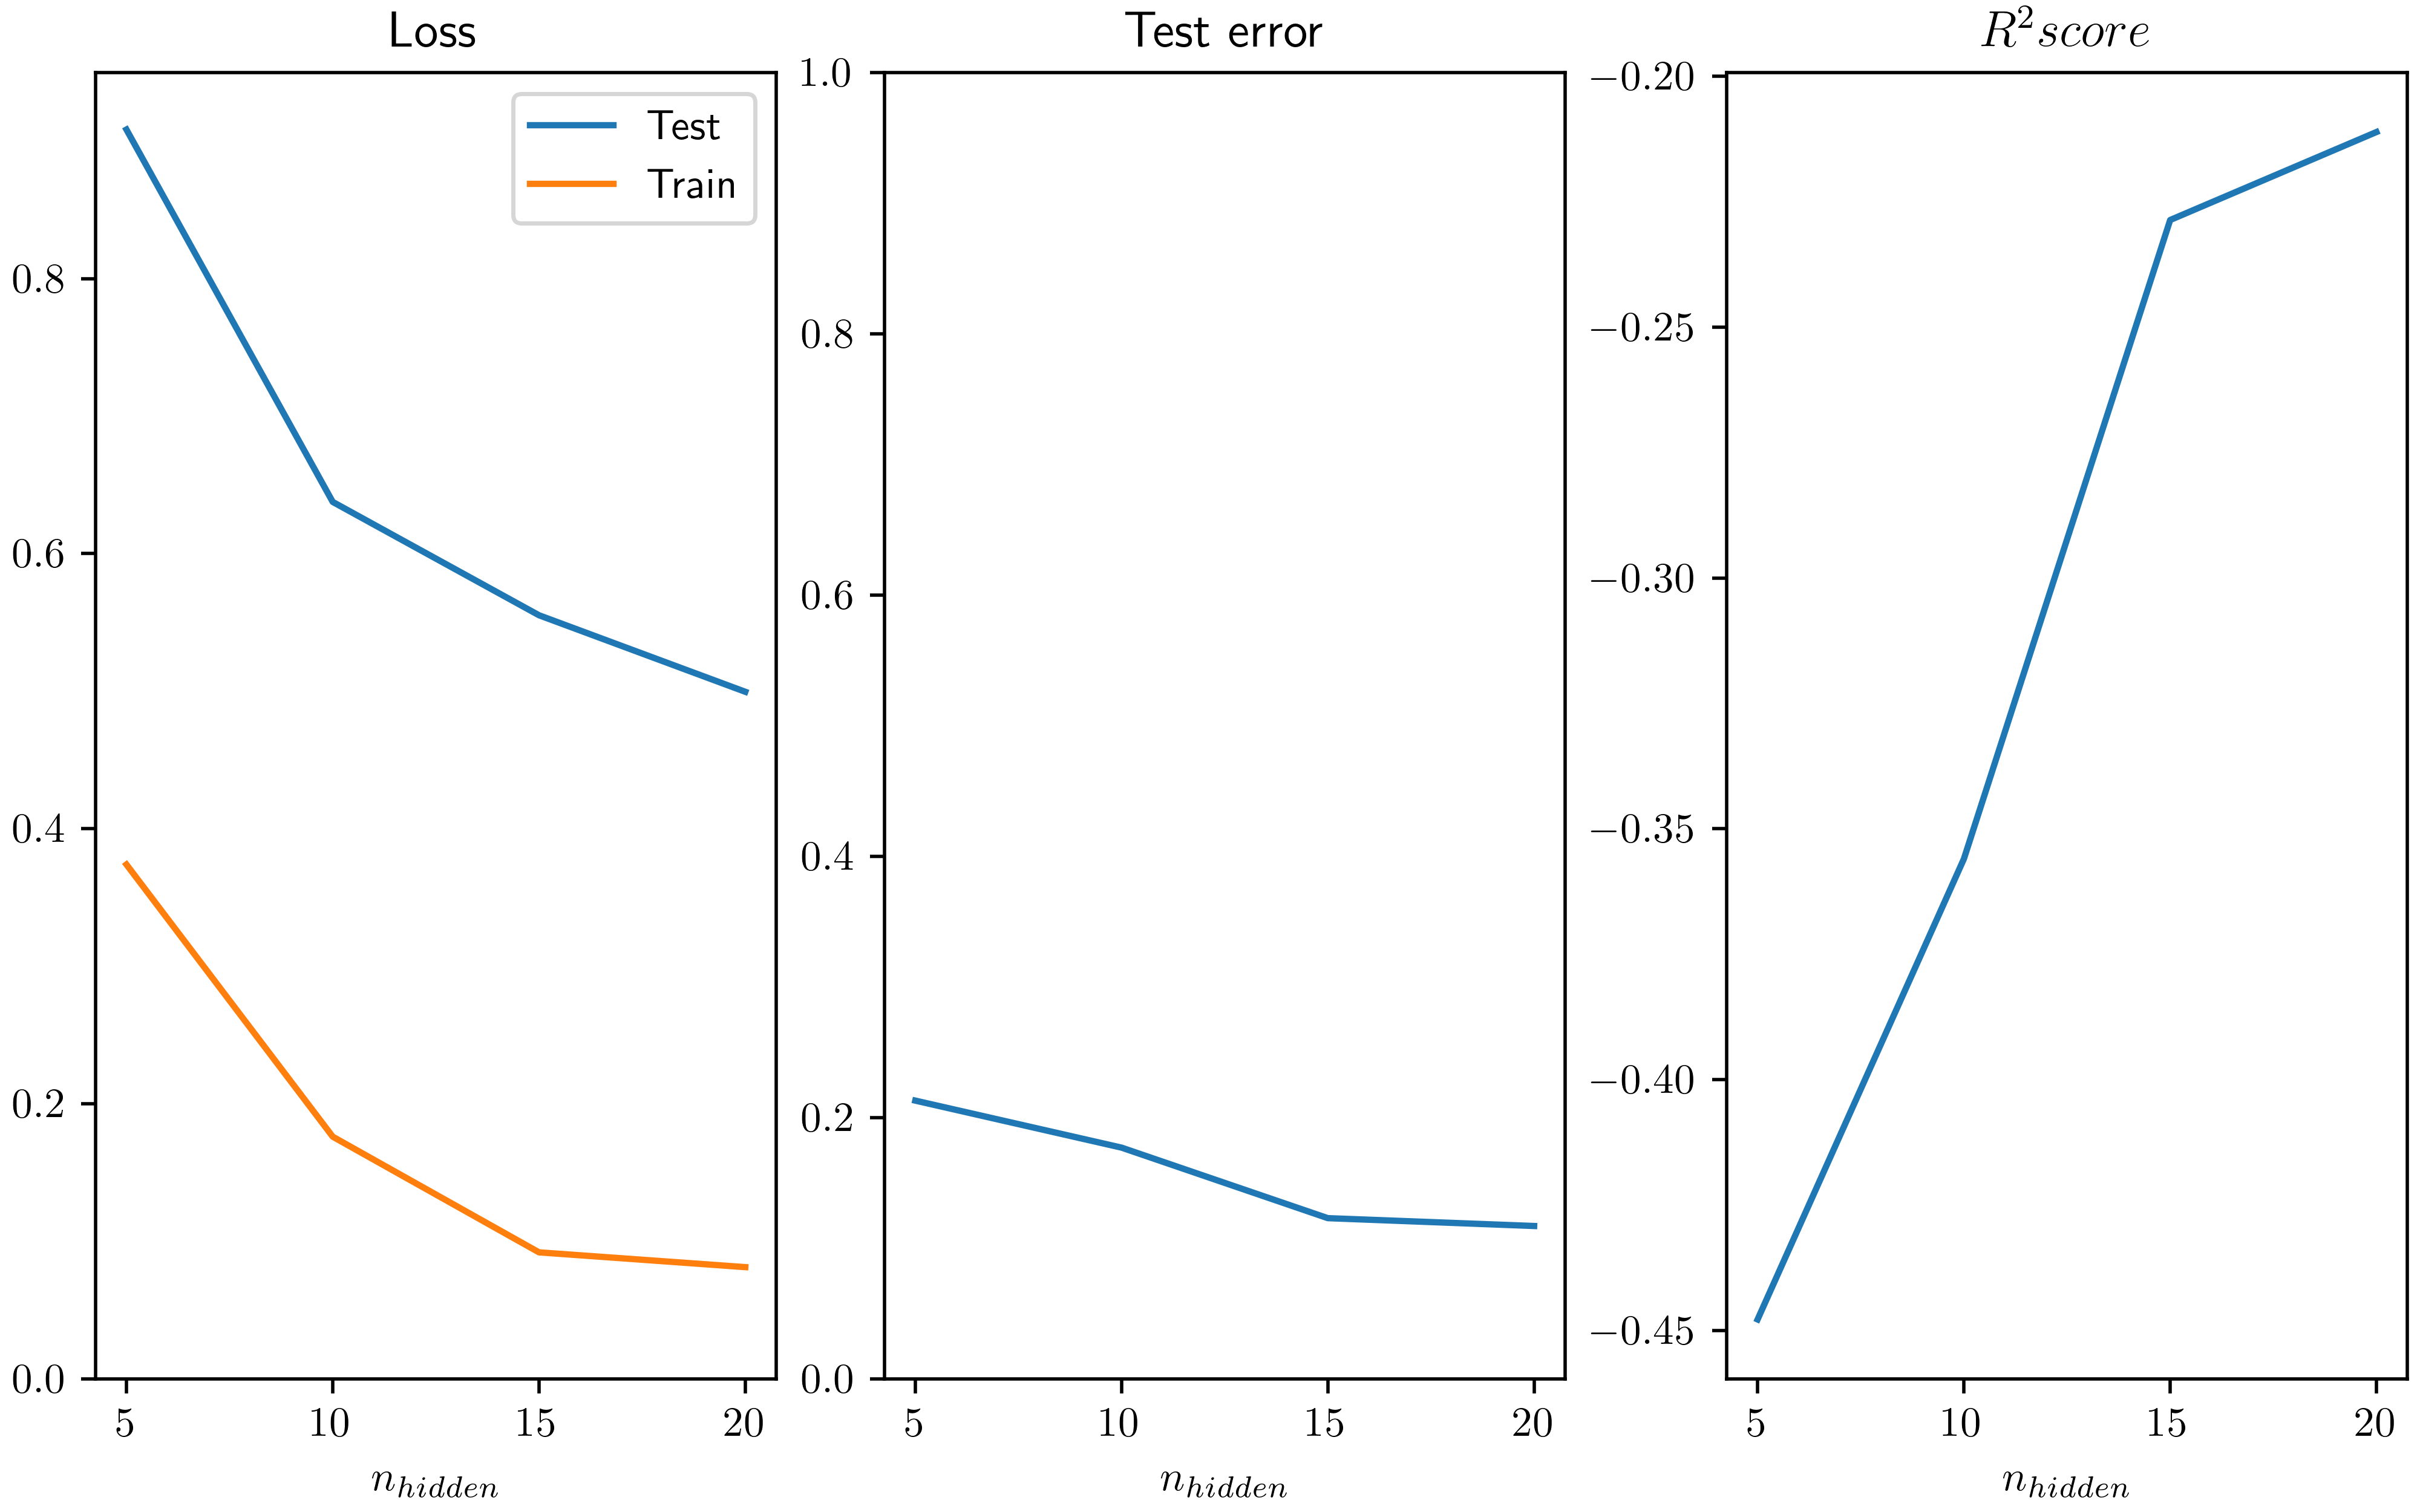
\includegraphics[width=0.95\textwidth]{fig_function_approximator}
    \caption[SNN learns to solve nonlinear regression task.]{SNN learns to solve nonlinear regression task. Networks of
    size $15-n_{hidden}-5$ neurons per layer were trained to predict the output of a separate multi-layer network of
    size $15-15-5$. Each network was trained on 500000 samples of the same teacher network while all somatic
    compartments received background noise with a standard deviation of $0.01$. To measure how much of the teacher
    network's variance is predicted by the dendritic error network, the $R^2$-score
    (\href{https://scikit-learn.org/stable/modules/generated/sklearn.metrics.r2_score.html}{sklearn.metrics.r2\_score})
    was measured for a final test run over 500 samples.}
    \label{fig-func-approx}
\end{figure}

As the task was found to be too easy when inputs to the teacher network were strictly positive (as is the case in the
self-prediction paradigm), inputs were drawn from a uniform distribution $U(-1,1)$. Note that (as is typical for many
neural networks), input neurons do not employ the nonlinearity $\phi$. Thus, in rate neurons inhibitory inputs are
transmitted directly and multiplied with synaptic weights. For spiking neurons, any negative injected current will
effectively inhibit spike generation. Thus, negative inputs can not be transmitted. To facilitate inhibitory stimulation
to the spiking network, a separate input layer population was required. This population was initialized with the
inverted weights of the excitatory population. An input vector was then separated, with positive values stimulating the
excitatory population and negative values stimulating inhibitory neurons. Due to this necessity, the spiking network
effectively had to learn an additional set of weights, which must be considered when assessing these results.

Results show that surprisingly small networks are capable of matching the teacher network approximately. However,
particularly for explaining the variance in the teacher network's output, at least an equally sized network  is
required. While the training task is complex, results stayed somewhat behind expectations, particularly for the network
of identical size ($n_{hidden} = 15$). Nonetheless, the network successfully learns the required input-output mapping
without resorting to just learning the mean output voltage. The results reported here suffer from a scaling error in the
NEST network. This error was alleviated later, leading to a final loss of $0.3$ and an $R^2$-score of $0.2$ for the
network with $n_{hidden} = 20$. The updated results could not be included due to time constraints, but show that the
network is generally more capable than this figure indicates. These experiments should be considered exploratory, as
fine tuning parameters and training on the large number of required samples was a time-consuming process.


\section{Apical compartment capacitance}\label{sec-c-m-api}

Next, an investigation was made into lowering apical- and FB errors of the spiking implementation. The hypothesis was
that a smoothing of apical compartment voltage would lead to a decrease in both errors. There is physiological data
supporting such experiments, as the surface area of pyramidal neuron dendrites outscales the soma by several orders of
magnitude \citep{Ishizuka1995}. According to the Neuronal cable theory, an increase in surface area should correspond to
an increase in overal membrane capacitance of a neuronal compartment \citep{Niebur2008}.


To test the effects of this, the Self-predicting experiment was repeated with numerous values for apical compartment
capacitance $C_m^{api} \in \{ 1, 250 \} pF$ (results not shown). The experiment showed that for $C_m^{api} = 50pF$,
apical error is almost halved ($0.0034 \rightarrow 0.0019$), and FB error is decreased by $80\%$ ($0.15 \rightarrow
    0.027$). These values are still at least an order of magnitude higher than those in the rate implementations, but mark a
substantial improvement. Increasing the parameter beyond this point further decreased apical error, but came at the cost
of slower convergence. Higher membrane capacitances in general increase the relaxation period of the entire network.
Thus, they require a highly undesirable increase in $t_{pres}$ for successful learning.

\begin{figure}[h]
    \centering
    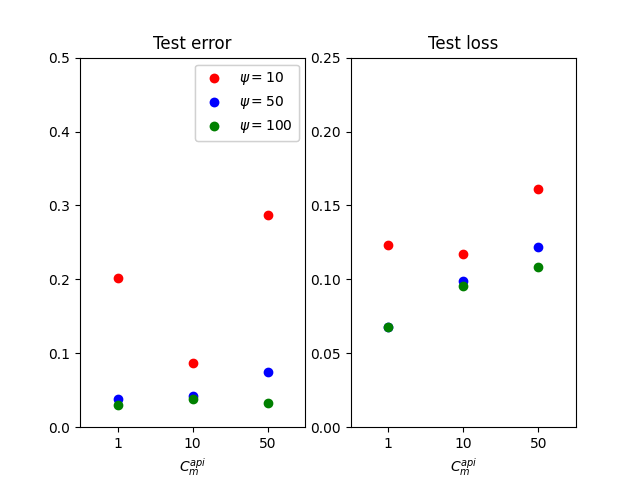
\includegraphics[width=0.9\textwidth]{fig_c_m_psi}
    \caption[Comparison of performance for different configurations of $\psi$ and $C_m^{api}$.]{Comparison of
    performance for different  configurations of $\psi$ and $C_m^{api}$. Networks were initialized with random weights,
    and trained for 750 epochs. Plasticity was enabled in all synapses ($\eta^{pi}=0.0025, \eta^{ip}=0.001,
        \eta^{up}_0=0.0025, \eta^{up}_1=0.00075, \eta^{down}=0$). Stimuli were presented for $t_{pres}=100ms$ to ensure that
    networks with higher apical capacitance (and therefore longer relaxation periods) were not disadvantaged too much. }
    \label{fig-c-m-psi}
\end{figure}

A secondary objective of training with different apical capacitances was to enable learning with lower $\psi$ and
therefore approach biologically plausible firing rates. To test this, training on the Bars dataset was performed under
different combinations of apical capacitance and $\psi$. Results of this experiment are shown in Fig. \ref{fig-c-m-psi}.

For $\psi=50$, increasing the membrane capacitance correlated directly with decreased performance. Curiously, the same
was true for $\psi=5$, but not necessarily for the intermediate value of $\psi=10$. In this special case, increasing
apical capacitance to a degree did improve performance. A possible explanation for this is, that a 'sweetspot' for
apical capacitance exists, in which the hypothesized stabilization of apical potential outweighs the drawbacks of
increased relaxation time. This parameter study remains inconclusive about this hypothesis, as too few combinations of
parameters are studied. Therefore, further experiments are required to determine if the utility of this parameter for
self-prediction can transfer to actual learning. I expect that increased apical capacitance combined with longer
stimulus presentation times could enable a decrease in $\psi$.


As basal compartments (and likewise FF error) did not fluctuate nearly as strongly, their capacitances were not
considered in the present work. While substantially smaller than the apical tree, their membrane capacitance should
similarly outscale the soma in future experiments.


\section{Imperfect connectivity}

Connectivity within cortical circuits, while structured, appears to subject to a high degree of randomness
\citep{potjans2014cell}. As noted before, one-to-one connections between pairs of neurons are therefore highly unlikely
\citep{whittington2019theories}. On the other hand, 'fully connected' populations of neurons likewise have not been
observed in electrophysiological \citep{thomson2002synaptic} and in-vitro \citep{binzegger2004quantitative} analyses of
cortico-cortical connectivity. Therefore, any network proclaiming to model the cortex must invariably be capable of
handling this imperfect connectivity.

\begin{figure}[h]
    \centering
    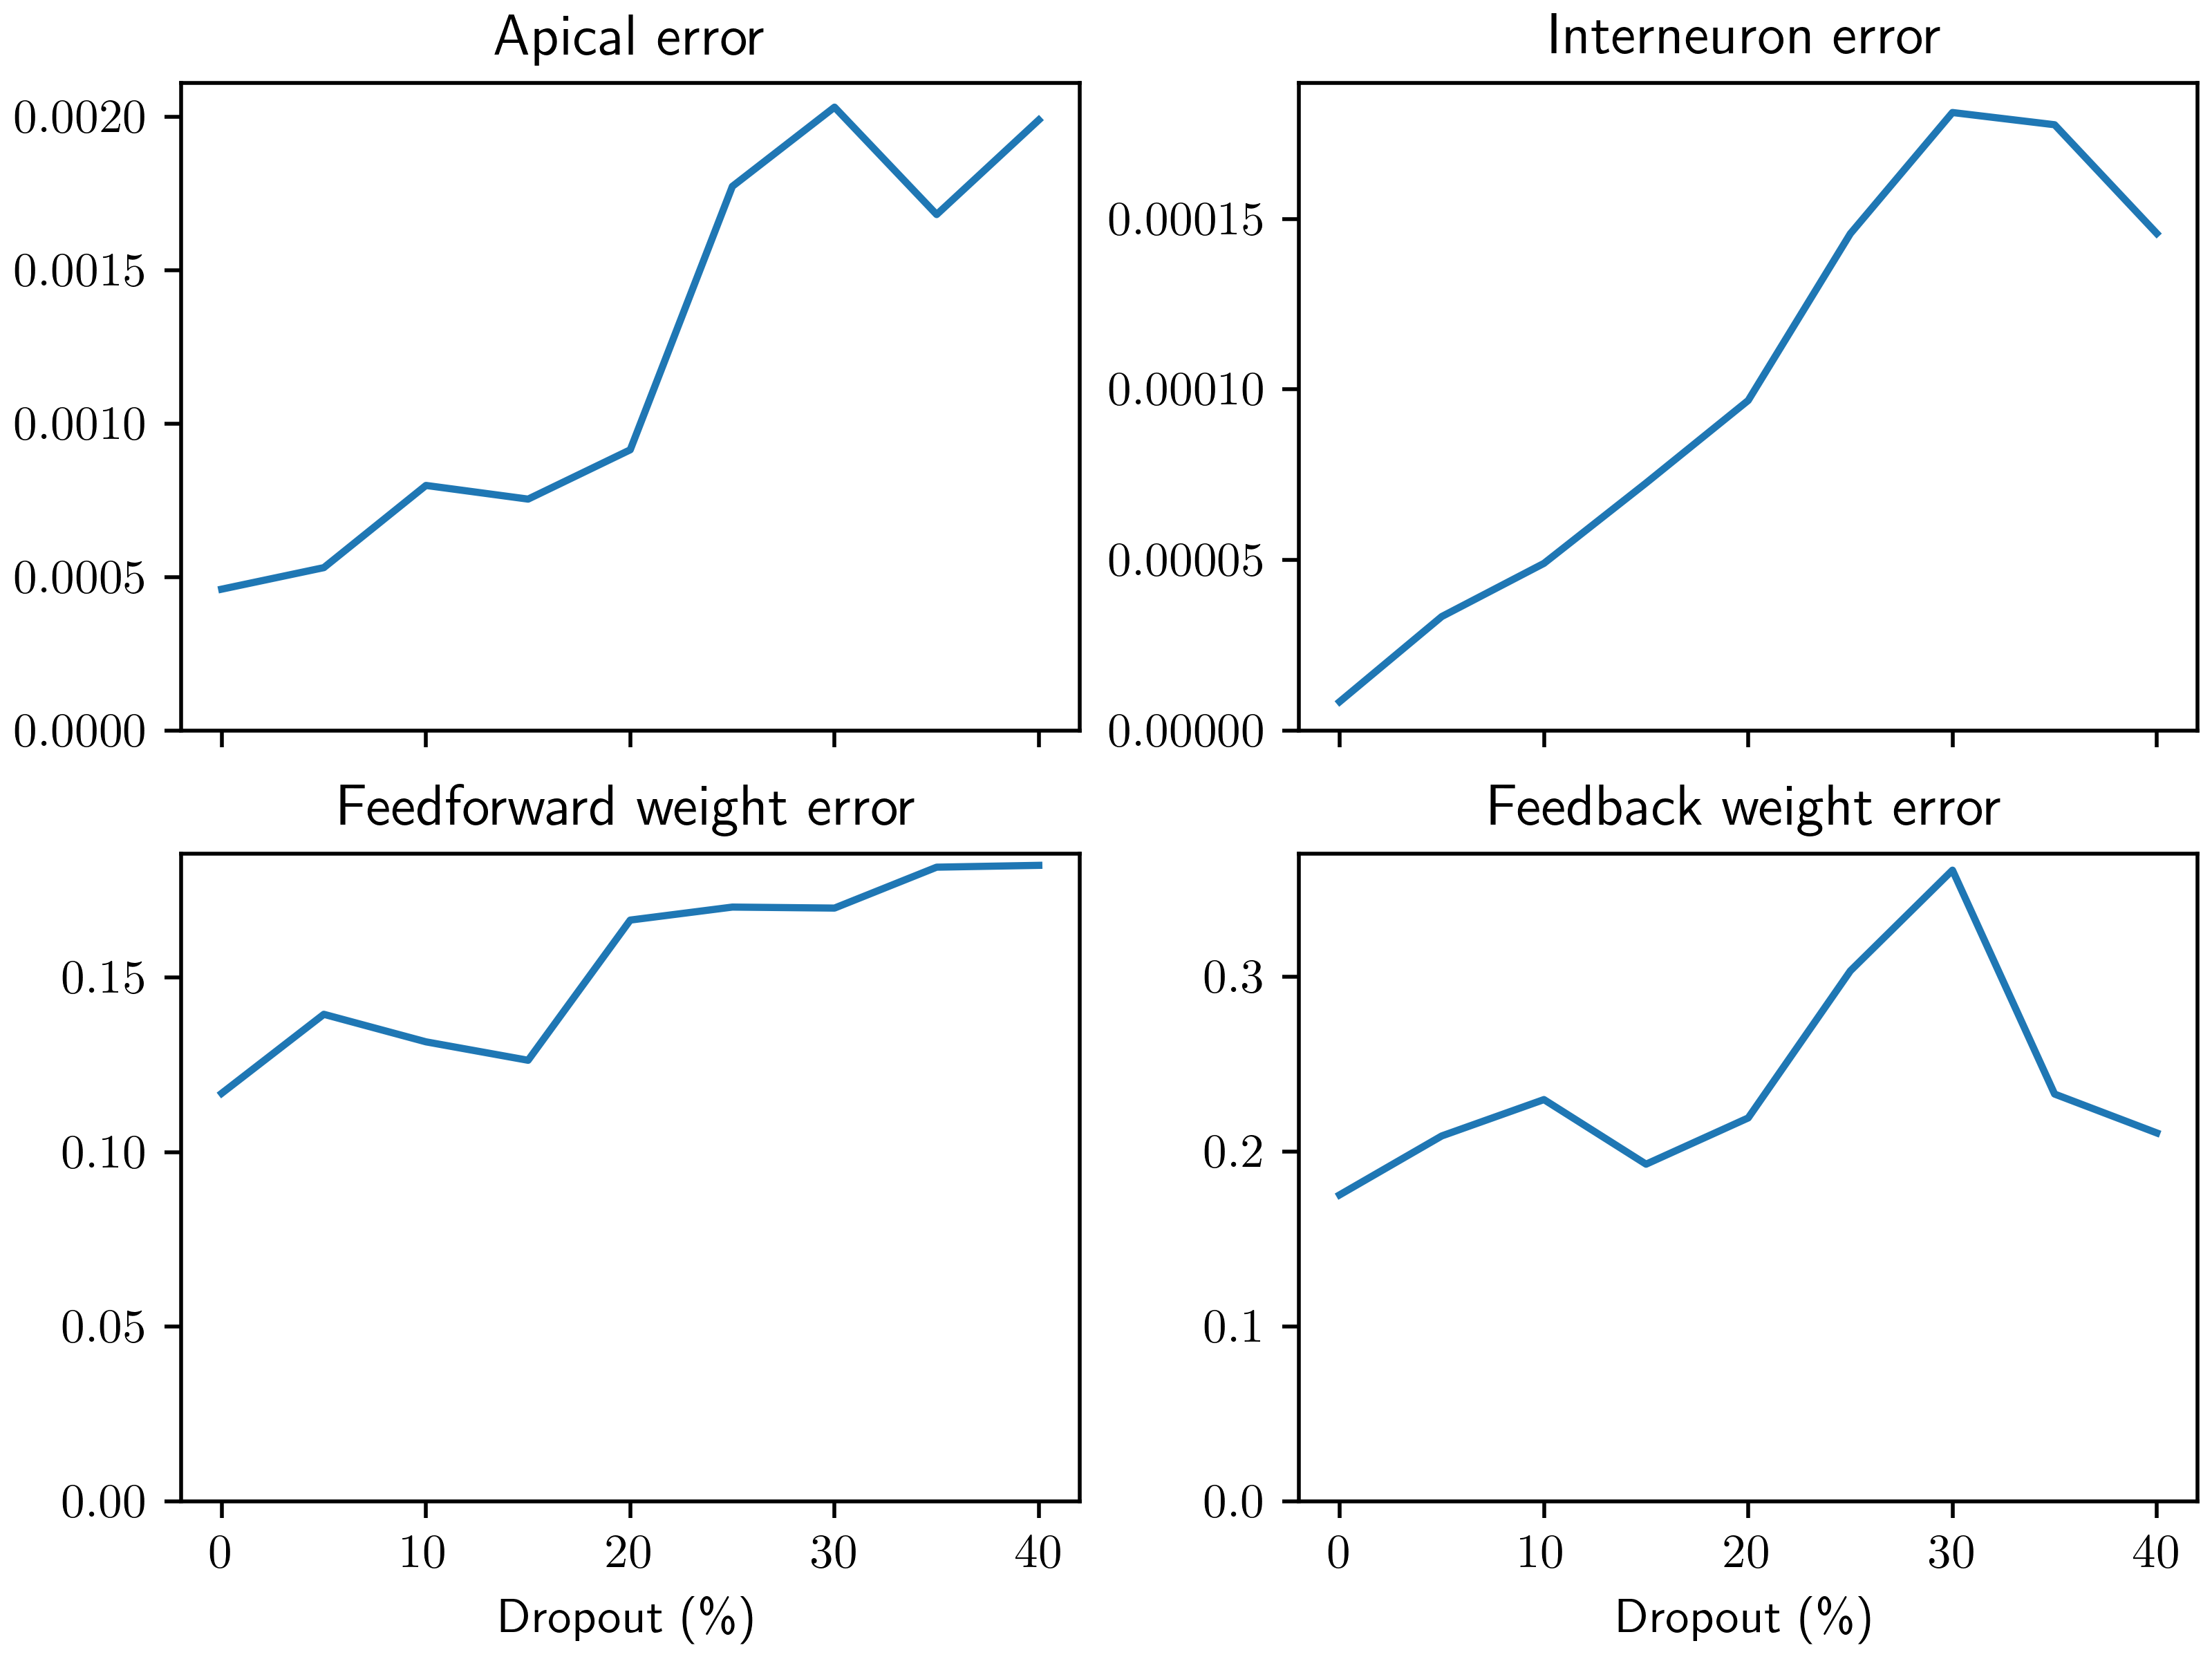
\includegraphics[width=0.9\textwidth]{fig_dropout}
    \caption[Error terms after training with synapse dropout]{Error terms after training with synapse dropout. Networks
        with $8-8-8$ neurons per layer were trained towards the self-predicting state, with different percentages of
        synaptic connections randomly removed. Experiments were performed with the rate-based network in NEST, each
        network was trained for 2000 epochs of 50ms each. Errors are averaged over 6 independent runs for each
        configuration.}
    \label{fig-dropout}
\end{figure}

To test if the dendritic error model fulfills this requirement, in a first step the self-prediction experiment was
repeated with neuron dropout. To simulate connection probabilities $p_{conn} \in {0.6, 1.0}$, an appropriate number of
synapses was deleted after network setup. To avoid completely separating two neuron populations, this deletion was
performed separately for each of the four synaptic populations.

As expected, removing synapses caused an increase in all four error metrics. Yet even with only 60\% of synaptic
connections present, the network manages to vastly improve from its random initialization. Weight errors are calculated
as mean squared errors over the two matrices, which requires matrices to contain data at every cell. Thus, to compute
these errors, weights of deleted synapses were set to zero in these matrices. This choice was made under the assumption
that a missing connection in an ideal self-predicting network would be matched by a zero-weight - or likewise absent -
synapse. These results indicate that the dendritic error rule is capable of compensating for absent synapses by
correctly identifying and depressing corresponding feedback connections (and vice versa). Through this mechanism, the
network is able to retain its self-predicting properties in spite of physiological constraints.


The extent of this capability was confirmed in SNN, by comparing performance on the Bars dataset of a control network to
a \textit{dropout network}. Both networks were initialized with random synaptic weights, and trained with full
plasticity ($\eta^{ip}_0 = 0.004, \eta^{pi}_0 = 0.01, \eta^{up}_0 = 0.01, \eta^{up}_1 = 0.003$) to best enable the
dropout network to compensate for missing synapses. The dropout network was initialized with $40$ instead of $30$ hidden
layer pyramidal neurons to counteract the deletion of $15\%$ of synapses per synaptic population. Both networks
performed very similarly, with the control network reaching $100\%$ accuracy somewhat faster (Epoch 140 vs. Epoch 200),
while the dropout network exhibited slightly lower test loss at the end of training (results not shown).

These results prove that the dendritic error model is capable of learning in spite of imperfect connectivity, which must
be expected to occur in the cortex. This sets it apart from the previous implementation of a predictive coding network
\citep{Whittington2017}, and further supports its biological plausibility.



\section{Separation of synaptic polarity}\label{sec-dales-law}


A dogma held in neuroscience for a long time now has been the notion that all neurons are either excitatory or
inhibitory, as dictated by their type (also known as Dale's law \citep{Kandel1968}). Several studies have since shown
that some neurons violate this law through co-transmission or specific release sites for different neurotransmitters
\citep{Svensson2019,Barranca2022}. Despite these findings, pyramidal neurons are still regarded to release exclusively
Glutamate, therefore being strictly excitatory \citep{gerfen2018long,spruston2008pyramidal,Eyal2018}. This has been
considered a rather weak criticism of the biological plausibility of Backprop \citep{Bartunov2018}. Yet given that the
dendritic error model explicitly proclaims to model pyramidal neurons, this concern is ripe to be addressed.

Initial experiments showed that restricting any synaptic population in the network to just one polarity, the network is
unable to reach the self-predicting state. Since the network relies on an intricate balance of excitation and inhibition
(e.g. to minimize Apical error), this result is to be expected. Thus, activity in any neuron must be able to have both
excitatory and inhibitory postsynaptic effects facilitated by appropriate synaptic weights. The most likely means by
which a neural network could achieve this separation is, to introduce an interneuron population of opposite polarity
between a population and its target.


To investigate to what degree the dendritic plasticity rule can deal with this constraint, an experiment was conducted:
A population of (excitatory) pyramidal neurons $A$  was connected to another population $C$ with plastic synapses that
were constrained to positive weights. In order to facilitate depression in $C$, each neuron in $A$ was also connected to
a single inhibitory interneuron in population $B$. This set of synapses was randomly initialized with positive weights and
non-plastic during this simulation. The interneurons in turn were connected to $C$ through plastic, inhibitory
connections. All incoming synapses at $C$ targeted the same dendritic compartment. When inducing a dendritic error in
that compartment, all plastic synapses in the network collaborated in order to minimize that error. When injecting a
positive basal error for example, the inhibitory weights ($B \rightarrow C$) decayed, while excitatory synaptic weights
($A \rightarrow C$) increased. Flipping the sign of that error injection had the opposite effect on weights, and
likewise cancelled the artificially induced error. This shows that a separation of synaptic polarity does not interfere
with the principles of the Urbanczik-Senn plasticity when depression is facilitated by interneurons.

\begin{figure}[h]
    \centering
    \begin{minipage}{0.2\textwidth}
        \textbf{a)}\par\medskip
        \centering
        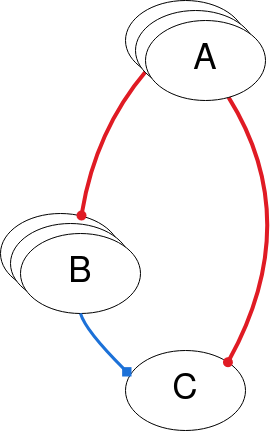
\includegraphics[width=0.9\textwidth]{fig_exc_inh_network}
    \end{minipage}\hfill
    \begin{minipage}{0.7\textwidth}
        \textbf{b)}\par\medskip
        \centering
        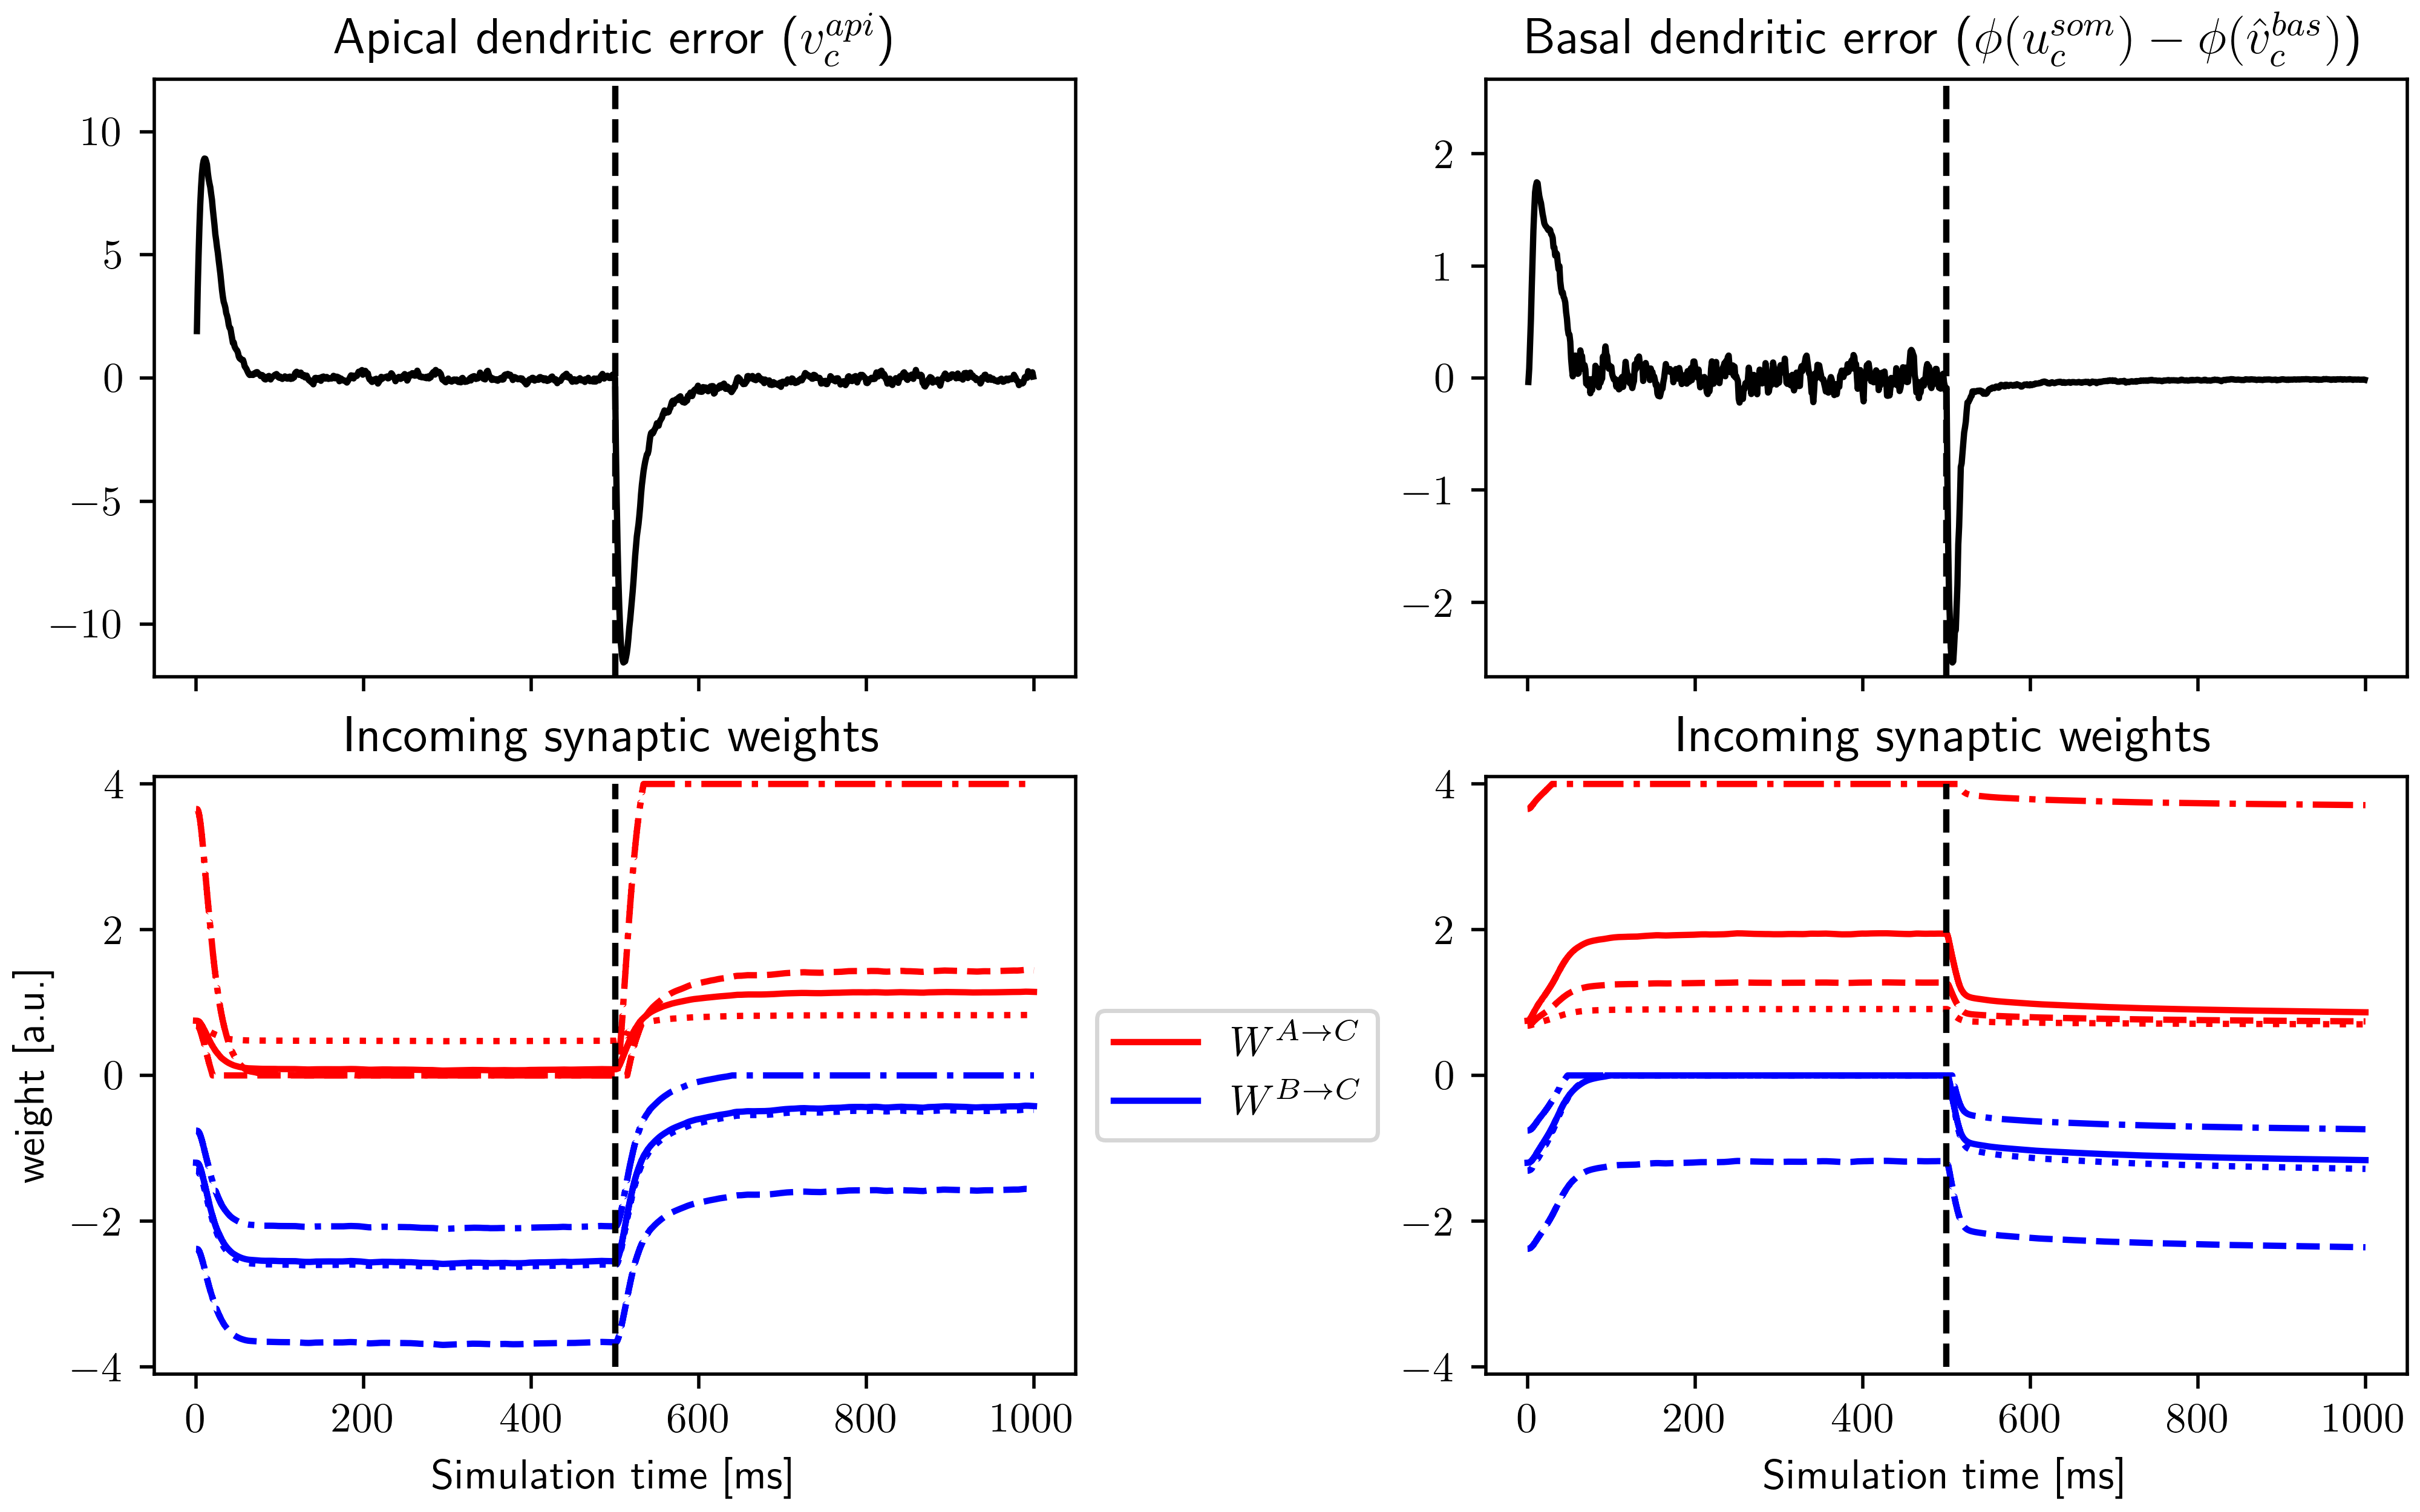
\includegraphics[width=0.9\textwidth]{fig_exc_inh_split}
    \end{minipage}
    \caption[Error minimization under biological constraints on synaptic polarity and network connectivity]{Error
        minimization under biological constraints on synaptic polarity and network connectivity. \textbf{a)} Network
        architecture. An excitatory population $A$ connects to a dendrite of Neuron $C$ both directly and through
        inhibitory interneuron population $B$. Only synapses $A\rightarrow C$ and $B \rightarrow C$ are plastic through
        dendritic error rules. Populations $A$ and $B$ are fully connected with random weights. \textbf{b)}
        \textit{Left:} All plastic synapses arrive at apical dendrites and evolve according to Equation
        \ref{eq-delta_w_pi}. \textit{Right:} Identical network setup, plasticity for synapses at basal dendrites
        (Equations \ref{eq-delta_w_up}, \ref{eq-delta_w_ip}). \textit{Top:} Dendritic error of a single target neuron.
        Errors of opposite signs are induced at $0$ and $500ms$ (vertical dashed line). \textit{Bottom:} Synaptic
        weights of incoming connections. All initial synaptic weights and input neuron activations were drawn from
        uniform distributions.}
    \label{fig-exc-inh-split}
\end{figure}

Yet, as criticized previously \citep{whittington2019theories}, the one-to-one connections between $A$ and $B$ are
untypical for cortical networks \citep{douglas2004neuronal,Gordon2010}. Hence, a second experiment was performed in
which neurons in populations $A$ and $B$ were fully connected. This decrease in specificity of the connections did not hinder the
error-correcting learning, as shown in Fig. \ref{fig-exc-inh-split}.

While error minimization is important, it does not necessarily imply that synaptic credit assignment is successful as
well. Numerous weight configurations are conceivable which could silence dendritic errors, but likely only a small
subset of them is capable of transmitting useful information. To prove that this nonspecific connectivity is compatible
with learning of complex tasks, it was introduced into the dendritic error network. The connection between interneurons
and pyramidal neuron apical dendrites was selected for the first test, as the employed plasticity rule had proven most
resilient to parameter imperfections previously. A network of rate neurons was set up and parametrized as described in
Section \ref{sec-le-tpres} ($t_{pres}= 50ms$). The Weights $w^{pi}$ were redrawn and restricted to positive values, and
a secondary inhibitory interneuron population was created and fully connected to both populations as described in Fig.
\ref{fig-exc-inh-split}. The inhibitory interneuron population was chosen to be 4 times as large as the target pyramidal
population, and $30\%$ of incoming excitatory connections were randomly deleted. The idea behind this was, to seed
interneurons which were to serve as inhibitory counterparts for individual excitatory partners. From this seeding, the
dendritic error rule could then ideally derive useful information about presynaptic activity.

The experiment was successful, as the network was able to learn successfully in competitive time (100\% accuracy after
200 Epochs) albeit to a higher final test loss (results not shown). These results show that the dendritic plasticity
rule is capable of correctly assigning credit to two separate populations when its inputs are much less sanitized.
Further experiments are required to show \textbf{A:} how large such an inhibitory interneuron population needs to be and
what role synapse dropout plays in it, \textbf{B:} whether this capability extends to the spiking implementation and
\textbf{C:} if all neuron populations in the network can be connected in this way to separate excitatory and inhibitory
pathways. Such experiments would allow for a closer investigation into how well the dendritic error network corresponds
to cortical connectivity - if at all. The novel neuron populations introduced by such experiments would themselves have
to have some cortical equivalent which they are to represent.



These results furthermore enable the conception a biologically plausible way for long-range pyramidal projections to
innervate neurons in another layer of the dendritic error model (i.e.\ in a different cortical area). The steps
required to facilitate this type of network are rather simple; A pyramidal neuron projection could enter a distant
cortical area and spread its axonal tree to innervate both pyramidal- and inhibitory interneuron dendrites. If these
interneurons themselves connect to the local pyramidal population, Dendritic errors with arbitrary signs and magnitudes
could be minimized. While this is unlikely to be the case in the cortex, pyramidal-to-interneuron weights do not need to
be plastic, as long as all synapses arriving at the target pyramidal population are.



\subsection{Interneuron nudging}

An easily overlooked connection of this network is the nudging signal from pyramidal neurons to their interneuron
sisters. These were deliberately not included in the previous dropout studies. If any interneuron was to not receive its
nudging signal, its incoming synapses would be unable to adapt their weights. As a result, both interneuron- and FF
error would fail to converge, in turn impeding apical error reduction. These one-to-one connections can  therefore be
considered the most important communication channels in the network. If there is no redundancy in the neurons, deleting
any of them breaks the network's learning scheme. Sacramento et al.\ claim that the interneurons of the network resemble
somatostatin-expressing (\textit{SST}) neurons. This is a reasonable assumption, as SST cells are ubiquitous in the
cortex and inhabit the same layers as pyramidal neurons. Furthermore, they share dense and recurrent synaptic
connections to these pyramidal neurons \citep{urban2016somatostatin}. Finally, they have been shown to receive top-down
instructive signals, which have been hypothesized to transmit prediction errors \citep{Leinweber2017}.

Several experiments similar to those on synaptic polarity were conducted in an attempt to replace these one-to-one
connections with more plausible connectivity schemes. Regrettably, none of them were able to retain the learning
capability of this network. Thus, these connections remain as perhaps the biologically most implausible aspect of the
dendritic error network. Further work is required to investigate if and how this constraint can be relaxed.



\section{Performance of the different implementations}\label{sec-benchmark}

As stated in \citep{Haider2021}, simulating large dendritic error networks with the full leaky dynamics quickly becomes
unfeasible. While the NEST simulator can be regarded as rather fast \citep{albada2018performance}, simulations on it by
design cannot employ batched matrix multiplication, as is typical in machine learning. Thus, by computing neuron updates
individually even in highly structured networks like this one, NEST was expected to perform worse than previous
implementations using PyTorch and dedicated GPUs. Yet not only did the NEST implementations compute rather slowly, the
spiking variant was the slowest across the board. To investigate the extent of this, as well as possible causes, several
benchmark experiments were performed. These tests were run on an \textit{AMD Ryzen Threadripper 2990WX} using 8 cores at
up to $3.0GHz$. All reported simulation times $t_{sim}$ are averaged over $5$ independent runs, and only measure the
time taken simulating (in seconds) without considering network initialization. \newline


\begin{figure}[h]
    \centering
    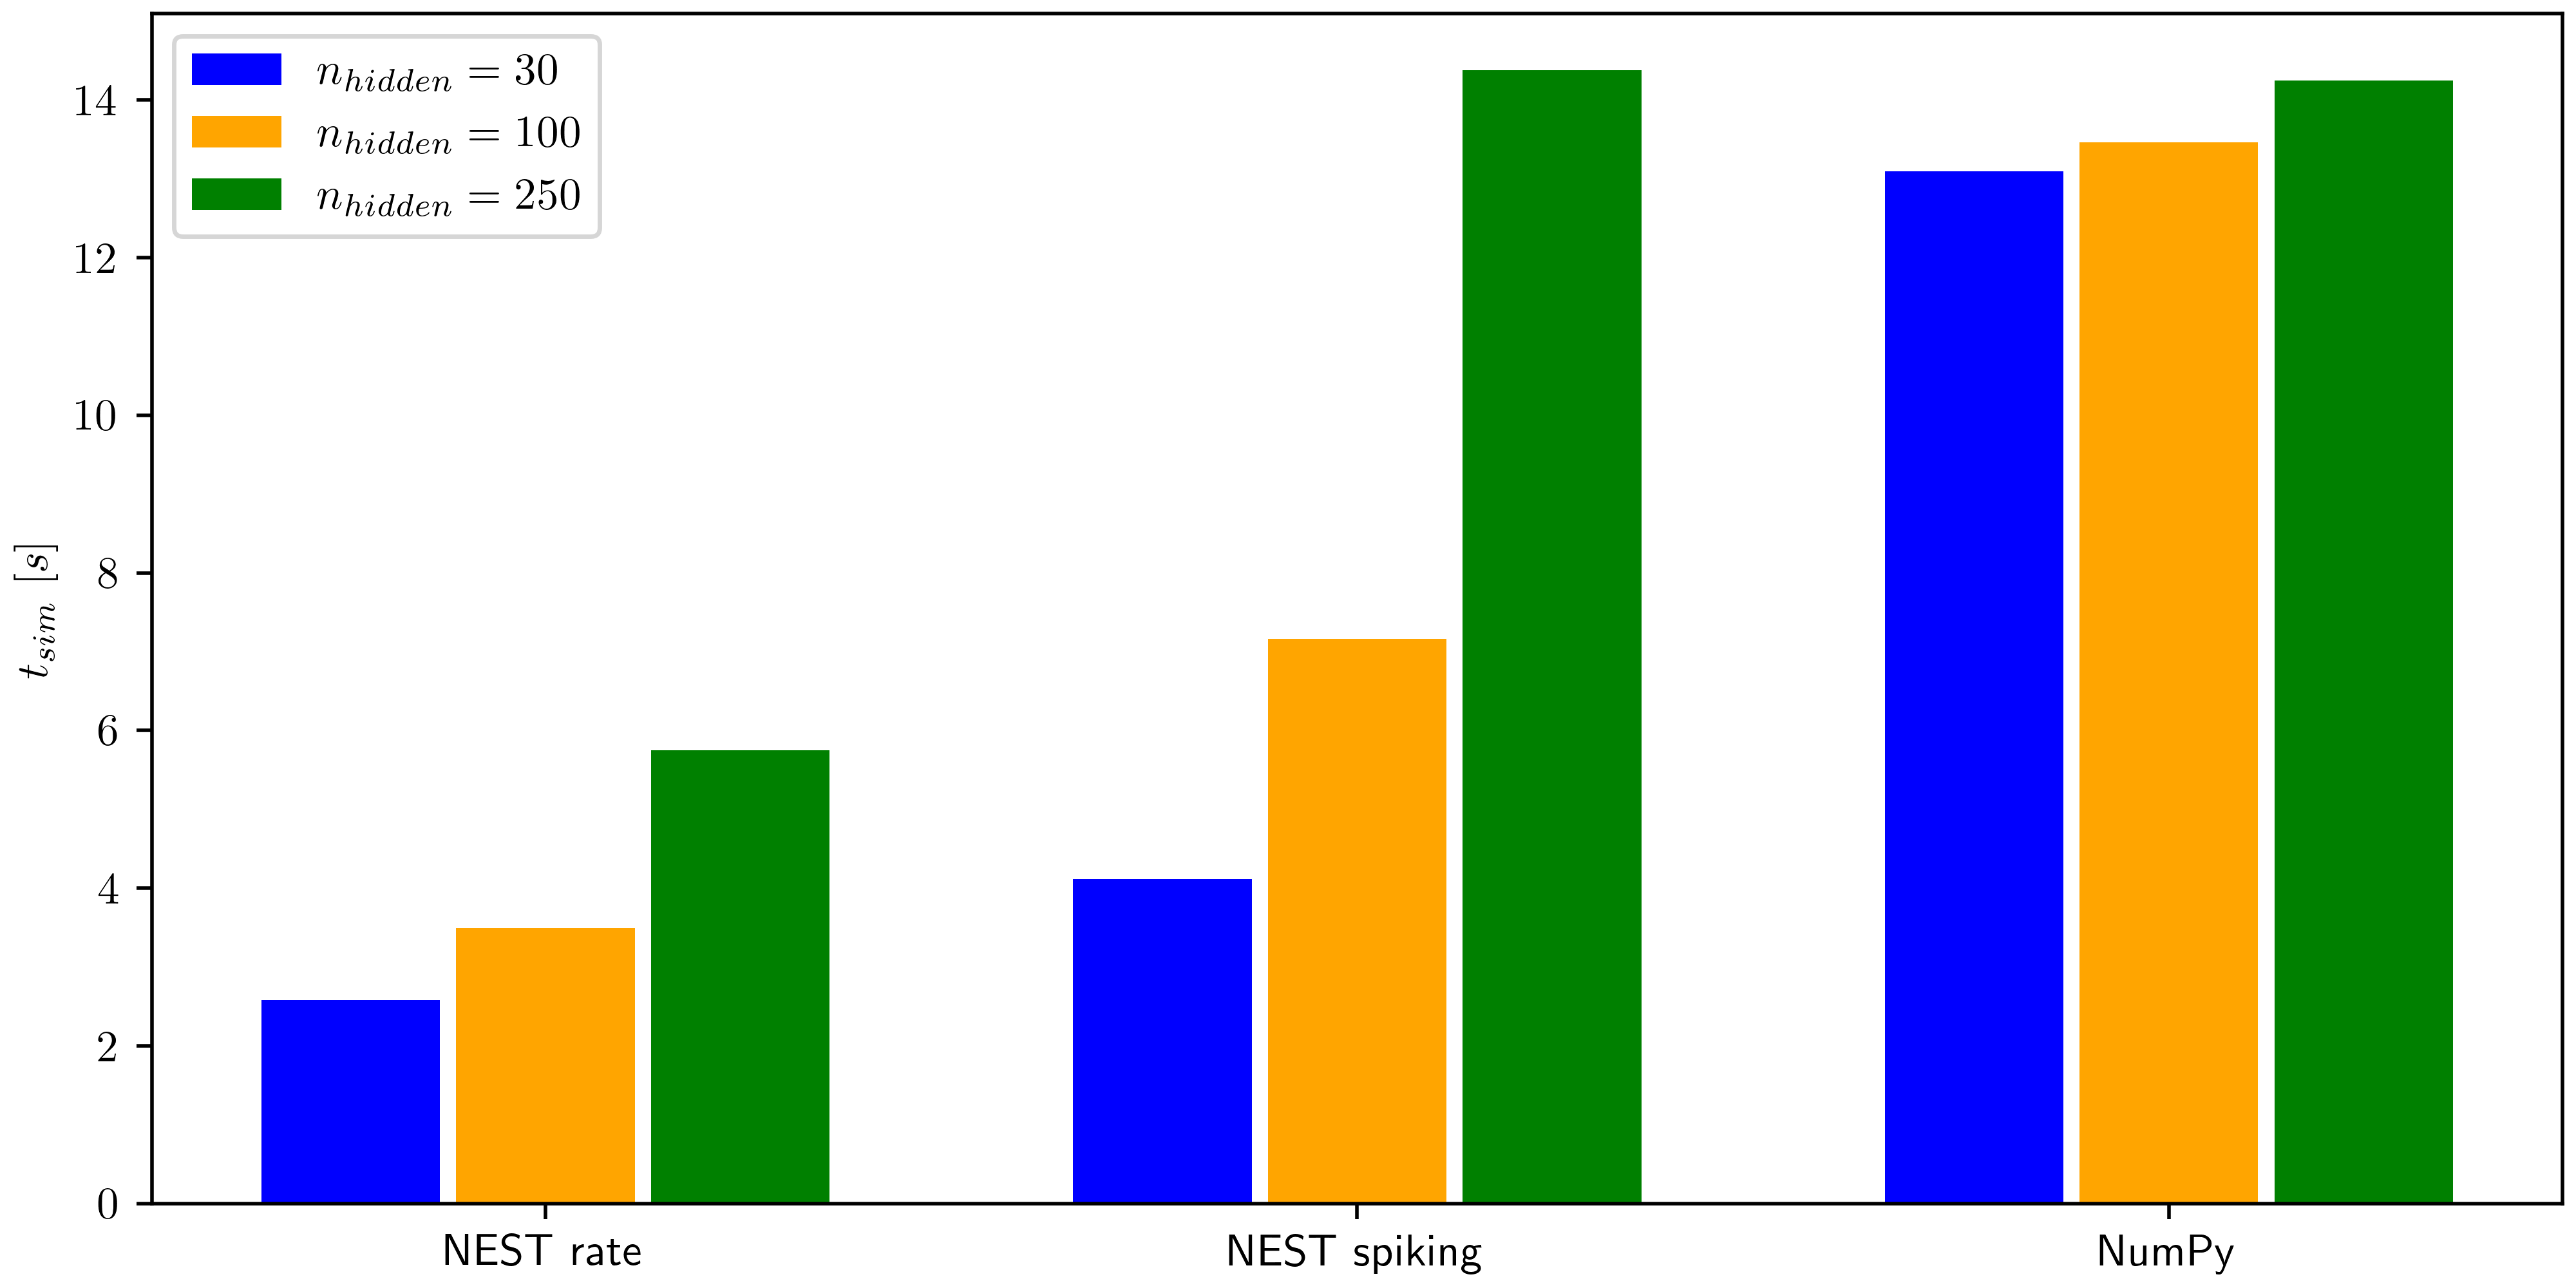
\includegraphics[width=0.95\textwidth]{fig_benchmark_n_hidden}
    \caption[Benchmark of the three implementations under different network sizes]{Benchmark of the three
        implementations under different network sizes. Networks of $[9, n_{hidden}, 3]$ neurons per layer  were
        instantiated with the same synaptic weights and trained for a single epoch of 10 stimulus presentations of
        $50ms$ each. $n_{hidden}=30$ was chosen as a baseline, as it is the default throughout all simulations on the
        Bars dataset.}
    \label{fig-benchmark-n-hidden}
\end{figure}


To compare how network size affects simulation time, all three implementations created for this project were trained on
10 examples of the Bars dataset with different numbers of hidden layer pyramidal neurons. The result of this comparison
is shown in Fig. \ref{fig-benchmark-n-hidden}.  The NEST implementation using rate neurons performed best in terms of
speed across the board. This result was slightly surprising, as the demand on the communication interface between
threads is very high, since all neurons transmit an event to each of their postsynaptic targets at every time step.

The NumPy variant is an outlier, and only listed here for completeness. It is the only variant running on a single
thread due to a limitation of NumPy. This could feasibly be improved greatly by using batched matrix multiplications, as
are provided for example by \texttt{PyTorch}. The original implementations do this, but for practical reasons the
Backend was changed here. Notably, this variant exhibits very little slowdown in response to an increase in network
size. It seems, that the vectorization of updates on a single thread scales better with network size than the
event-based communication performed by NEST.

Not only is the spiking variant of this model slower than the rate version, it also scales worse with network size.
Simulation time between $100$ and $250$ hidden layer neurons doubled, compared to an increase of $1.6$ for the rate
network. The Difference between the two was even greater when simulating on an office-grade processor (\textit{Intel
    Core i5-9300H} @ $2.40GHz$, results not shown). Several insights about the comparatively poor performance can be deduced
from a first approximation: The most likely causes for increased compute speed are the communication of events and the
synaptic plasticity rules. Updates to the neuron state are unlikely to be responsible for the worse performance, as both
neuron models are modelled almost identically. These assumptions were tested experimentally.



\begin{figure}[h]
    \centering
    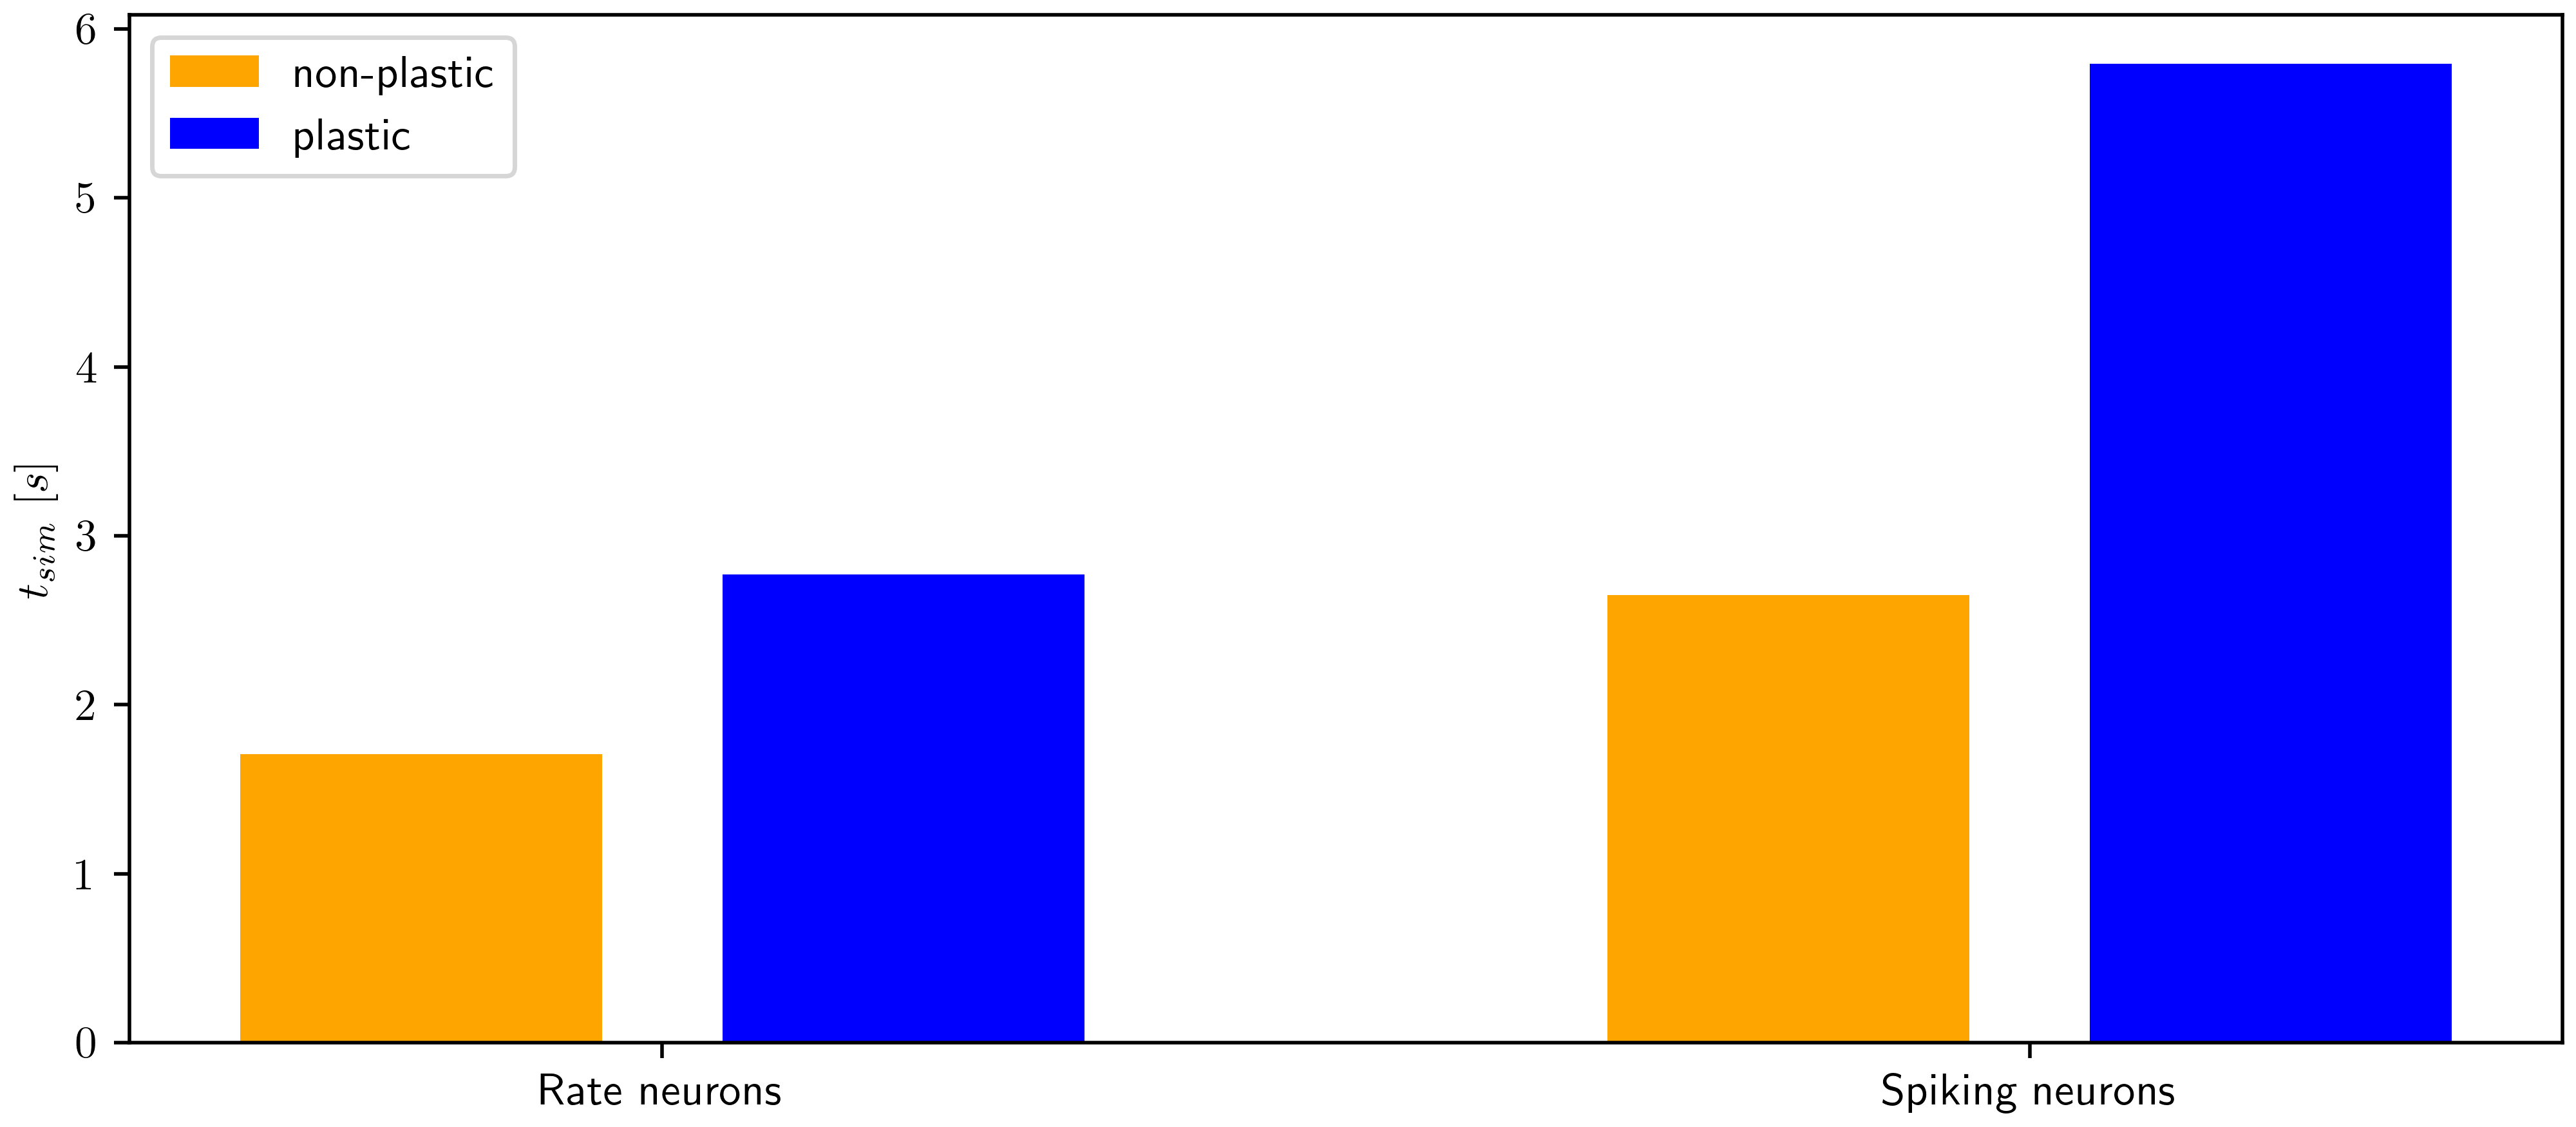
\includegraphics[width=0.8\textwidth]{fig_benchmark_plasticity}
    \caption[Benchmark of both NEST implementations with plastic and non-plastic synapse types]{Benchmark of both NEST
        implementations with plastic and non-plastic synapse types. Deep networks of $300-200-100-10$ pyramidal neurons
        per layer were stimulated with 5 samples of random input $\in\{0,1\}$ for $10ms$ each. synaptic weights were
        initialized between $\{-0.1, 0.1 \}$ to avoid overstimulation of individual neurons. In the plastic paradigm,
        all synapses except for feedback weights $w^{down}$ were plastic with very low learning rates $\eta =
            10^{-10}$.}
    \label{fig-benchmark-plasticity}
\end{figure}


To assess the impact of synaptic updates on computation time, both variants were simulated once with plastic, and once
with static synapses. The simulation environment is set up to model synaptic populations with zero-valued learning rates
as non-plastic synapses (\texttt{static\_synapse} and \texttt{rate\_connection\_delayed} respectively). Thus, by setting
learning rates to zero, it was possible to simulate an entire network without spending any time on synaptic updates.
Results of this experiment are shown in Fig. \ref{fig-benchmark-plasticity}.

As expected, synaptic updates in the spiking network are responsible for a much larger proportion of total simulation
time than in the rate network. A much less anticipated result was that spiking networks are considerably slower even
when plasticity is turned off. This is surprising, as neuron models are almost identical except for some added
complexity in the spike generation process. This added complexity includes drawing from a Poisson process, which might
be time-costly depending on the underlying implementation. Another possible reason might be added complexity associated
with SpikeEvents in general, which update some postsynaptic variables not employed for this model. Further work is
required to more rigorously determine the reasons for this poor performance.\newline

\noindent To investigate the degree to which synaptic plasticity and spike transmission in general contribute to
computational cost, two more experiments were conducted. Training durations under different values for the scaling
parameter $\psi$, as well as with different numbers of threads were recorded. Results are shown in Fig.
\ref{fig-benchmark-threads-psi}.

\begin{figure}[h]
    \centering
    \begin{minipage}{0.5\textwidth}
        \textbf{a)}\par\medskip
        \centering
        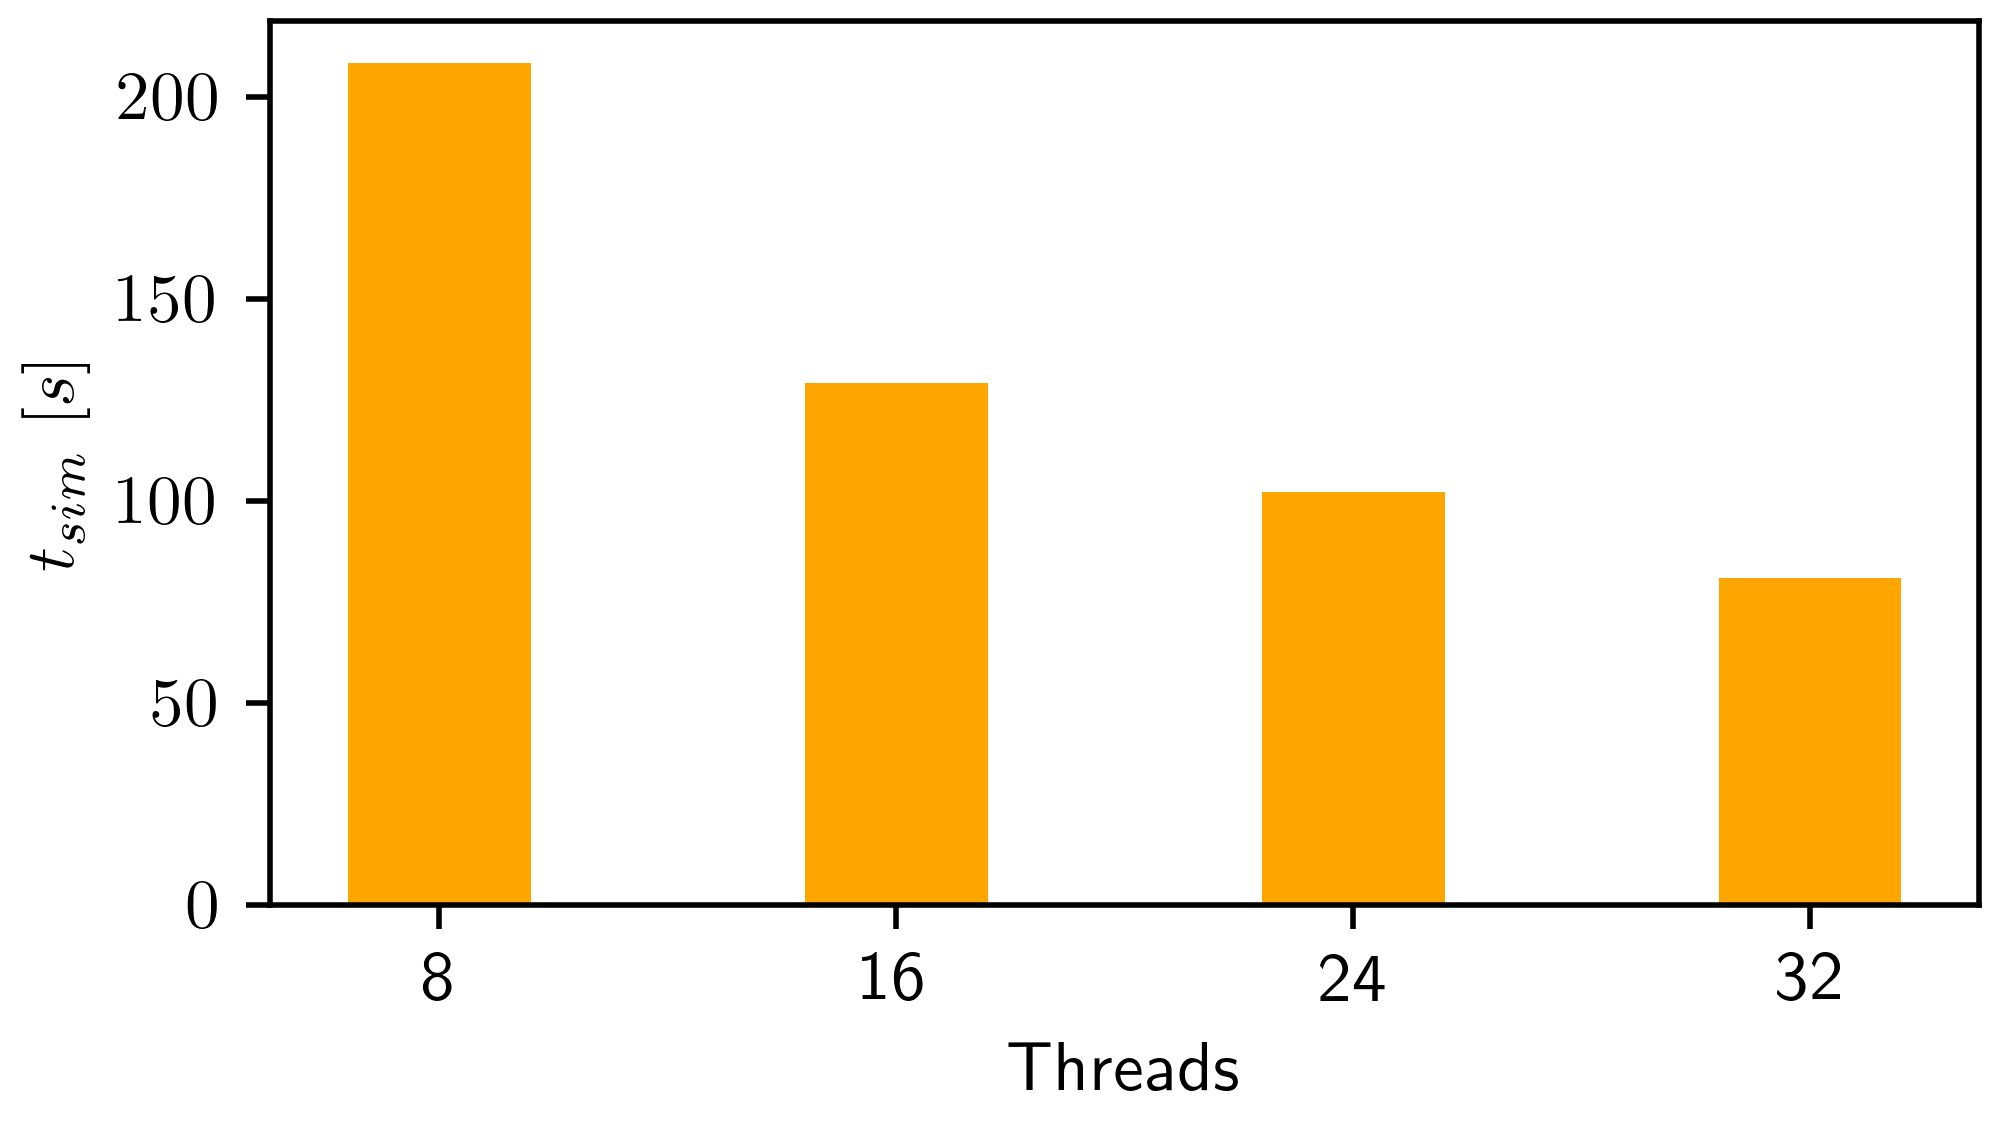
\includegraphics[width=0.95\textwidth]{fig_benchmark_threads}
    \end{minipage}\hfill
    \begin{minipage}{0.5\textwidth}
        \textbf{b)}\par\medskip
        \centering
        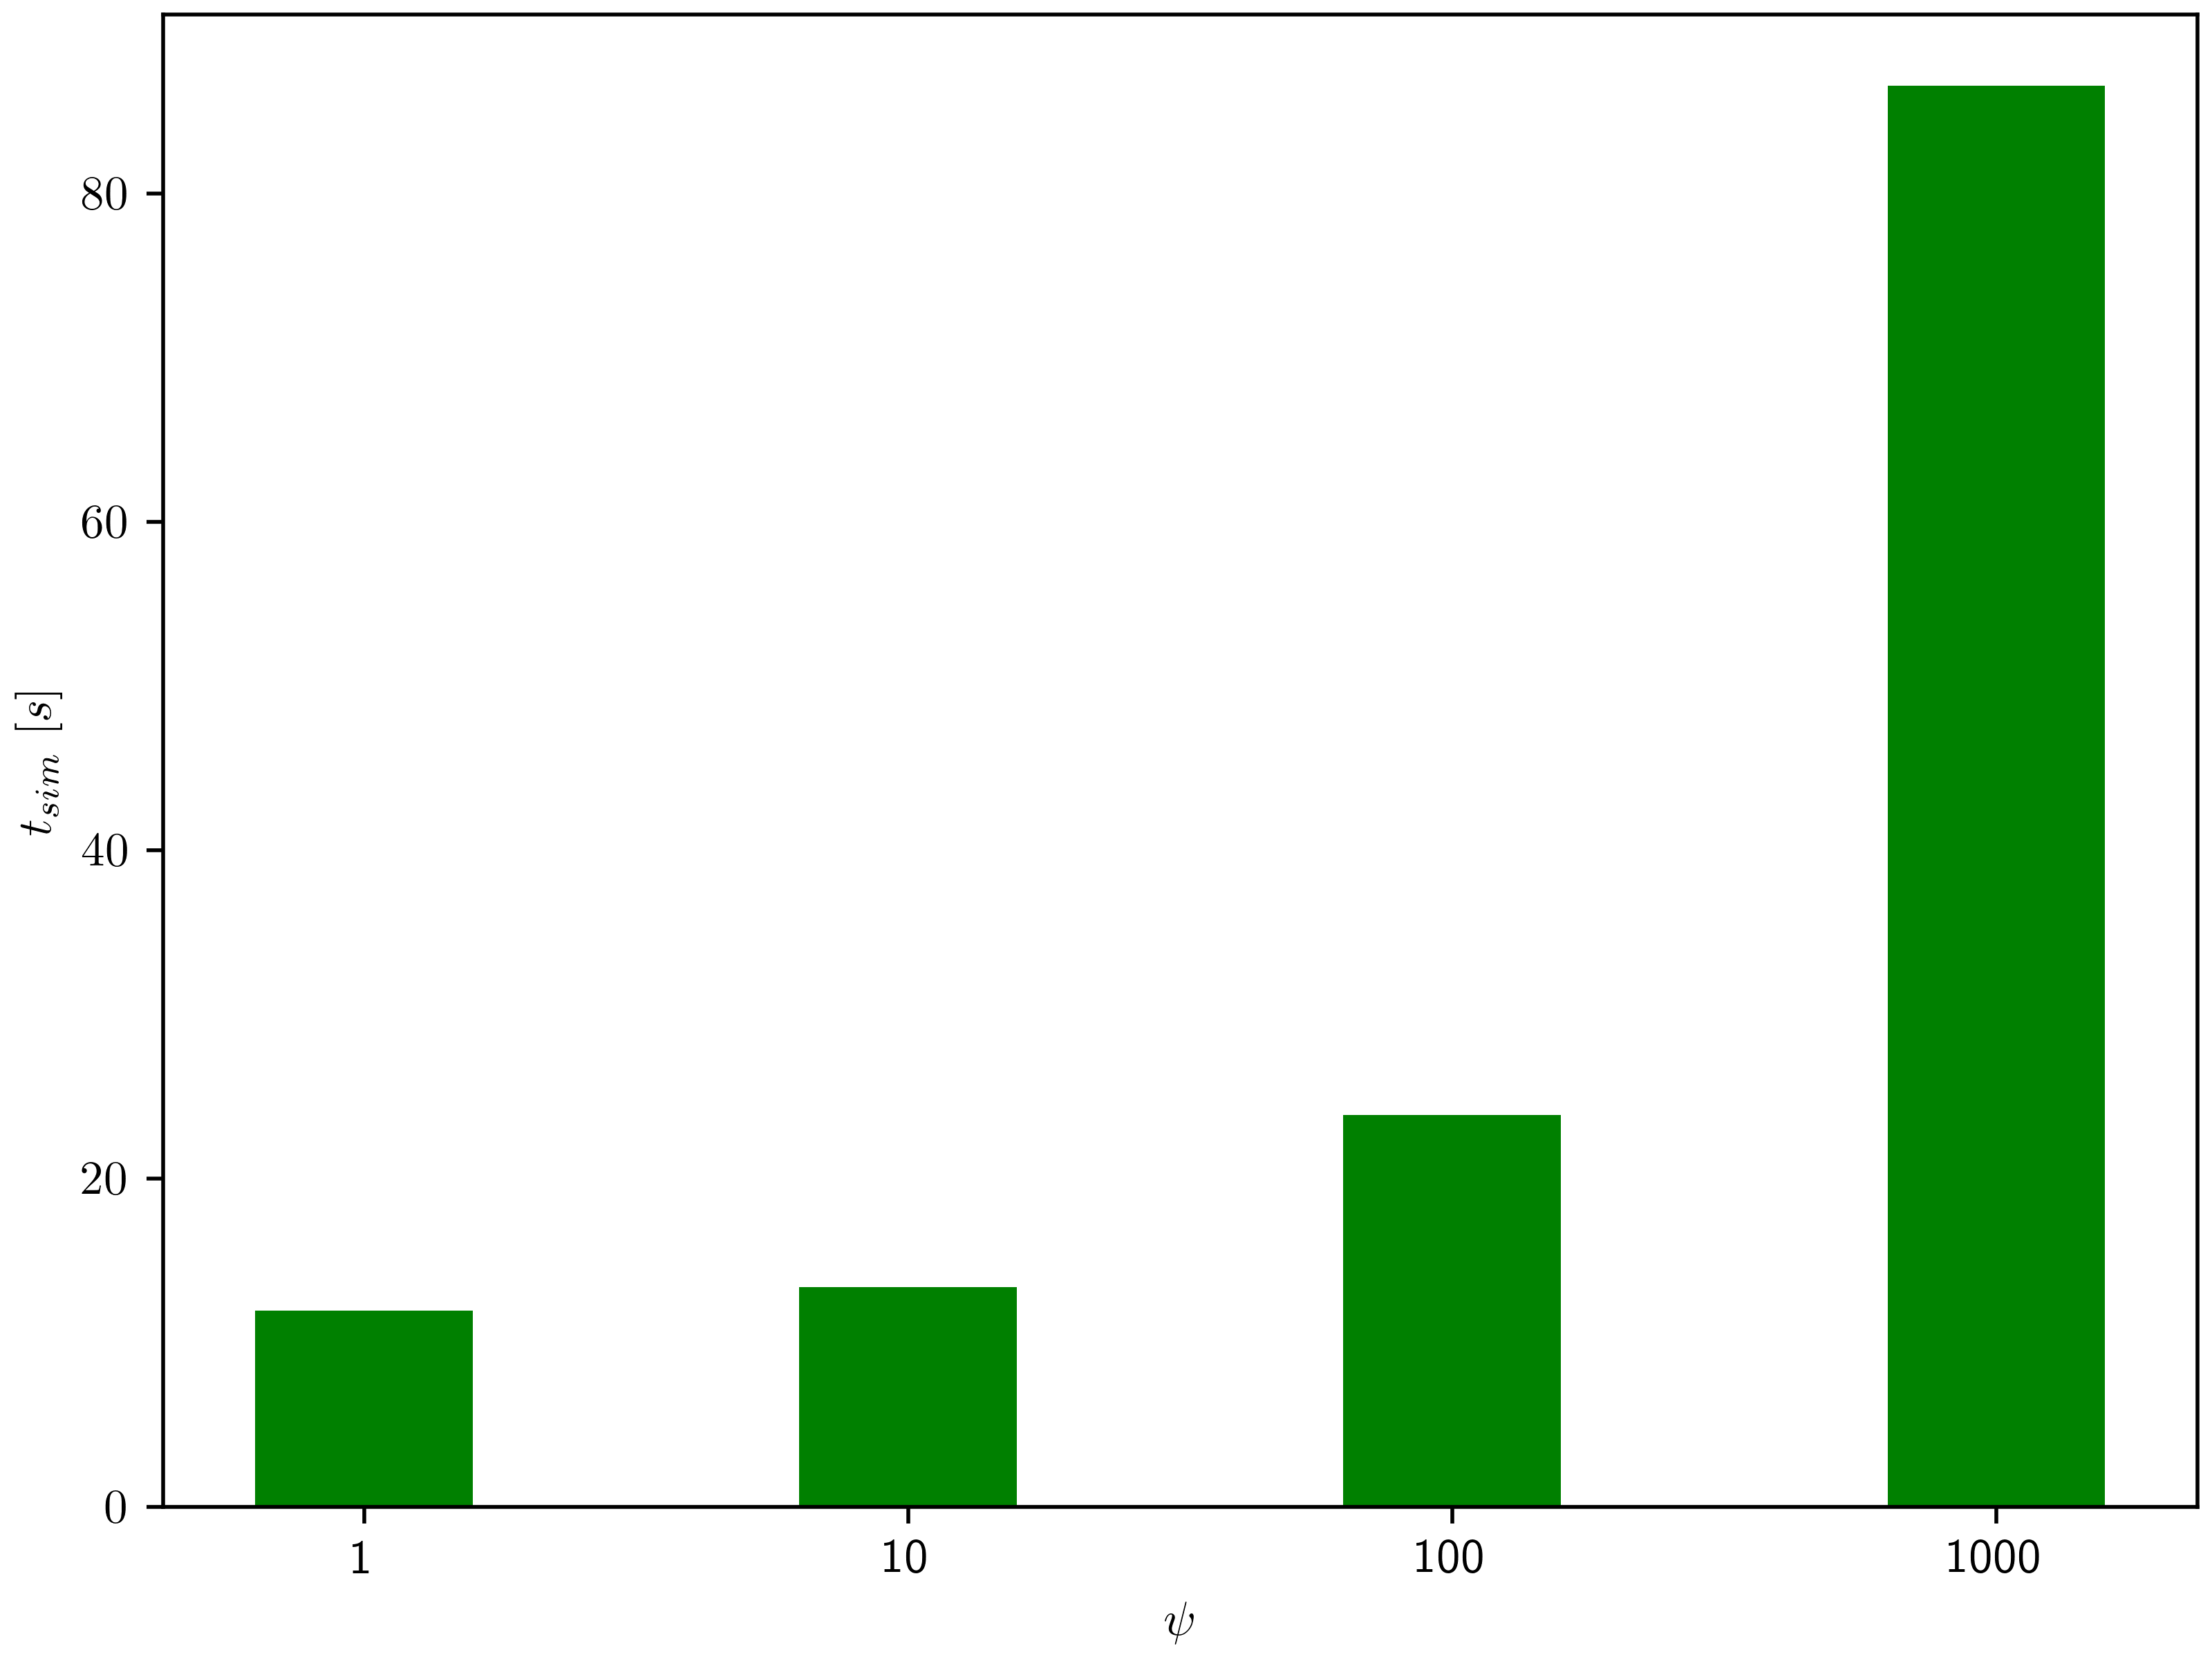
\includegraphics[width=0.95\textwidth]{fig_benchmark_psi}
    \end{minipage}
    \caption[Benchmarks for the spiking implementation]{Benchmarks for the spiking implementation. \textbf{a)}
        Simulation on the MNIST dataset for a network of $784-300-100-10$ neurons and $\psi=250$ on different numbers of
        threads. 10 samples were presented for $50ms$ each, and weights were drawn randomly from a uniform distribution
        $ \{-0.1, 0.1\}$. \textbf{b)} Training of a default network on the Bars dataset using different values of the
        scaling parameter $\psi$. All simulations use 8 threads.}
    \label{fig-benchmark-threads-psi}
\end{figure}

Simulating a large network on an increasing number of threads highlights the diminishing returns gained by spreading out
the simulation of NEST neurons. While initial speedup is high, at some point the benefit of parallelizing neuron updates
is counteracted by the need to communicate more events across threads. It is to be expected that for even higher
parallelization simulation time will begin to increase for this network size.

The second figure shows that reducing $\psi$ much lower will likewise lead to diminishing returns. On the other hand,
increasing it in the hopes of improving learning performance comes at a stark cost to simulation time. These results
should inform future experiments on increasing efficiency through parametrization.

\section{Pre-training}

One of the two major criticisms of the network noted in \citep{whittington2019theories} is the requirement for
pre-training (cf. Supplementary Table \ref{tab-wb-models}). By this, the authors mean the initialization to the
self-predicting state from which most simulations are started. The original paper implicitly considers three different
learning configurations: In the first one, the network starts from the self-predicting state and only feedforward
weights are plastic (cf. Sec. \ref{sec-le-tpres}). In the second one, the network starts from random weights and $Intn
    \rightarrow Pyr$ synapses are plastic, so they can minimize FB error. The third variant, in which feedback $Pyr
    \rightarrow Pyr$ weights are plastic, is not considered here. An experiment was conducted comparing performance of the
first two variants while training on the Bars dataset. These experiments showed that training was only marginally
slower, but led to identical loss (results not shown). While initializing the network to a self-predicting state does
give it a slight 'head-start', this is by no means a condition for successful learning.

Yet the nature of this pre-training is more important to this argument. Training the network towards the self-predicting
state does not require any kind of structured input, let alone targets for activation. The network is driven towards
this state purely by noise injection at the input layer. Therefore, any kind of input can serve to 'train' the network
to self-predict - be it a side product of other cortical processes or sensory stimuli for which no target has yet been
developed. It has for example been shown that background noise is ubiqutous in cortical circuits, particularly during
resting states, i.e.\ in the absence of an explicit task \citep{Deco2009}. As such noise therefore seems trivial for the
brain to generate (perhaps unavoidable), the self-predicting state might even be the default rather than the exception.
For these reasons, the requirement for pre-training is considered a rather weak criticism of the model's biological
plausibility.


\section{Behavioral timescale learning}

As a final experiment, the extent to which the network can handle learning on biological timescales was investigated.
One criticism occasionally aimed at Backprop is the requirement for instructive signals to be available immediately
\citep{Bartunov2018}. The assumption is, that an agent in the real world would select an action, and be informed about
the consequences only after some delay. Learning algorithms should therefore be capable of handling delayed instructive
signals.

Furthermore, all membrane potentials and synaptic weight derivatives of the dendritic error network are reset after each
stimulus presentation. This procedure ensures that residuals from the previous run do not interfere with learning of a
subsequent stimulus. It was confirmed experimentally that networks fail to learn when this reset is not performed after
every training sample (results not shown).

Two additions were made to the model to confirm that it is capable of learning without these constraints. First, the
target activation was delayed to be first injected $5ms$ after the stimulus. This serves to ensure that  that learning
does not rely on simultaneous presentation of stimulus and target. Secondly, instead of manually resetting membrane
potentials, the network was allowed to relax after each training sample. During this relaxation period  (termed
\textit{soft reset}), the network is simulated for $15ms$ without any current injections. A training comparison between
a vanilla network and these two additions is shown in Fig. \ref{fig-idle-time}.


\begin{figure}[h]
    \centering
    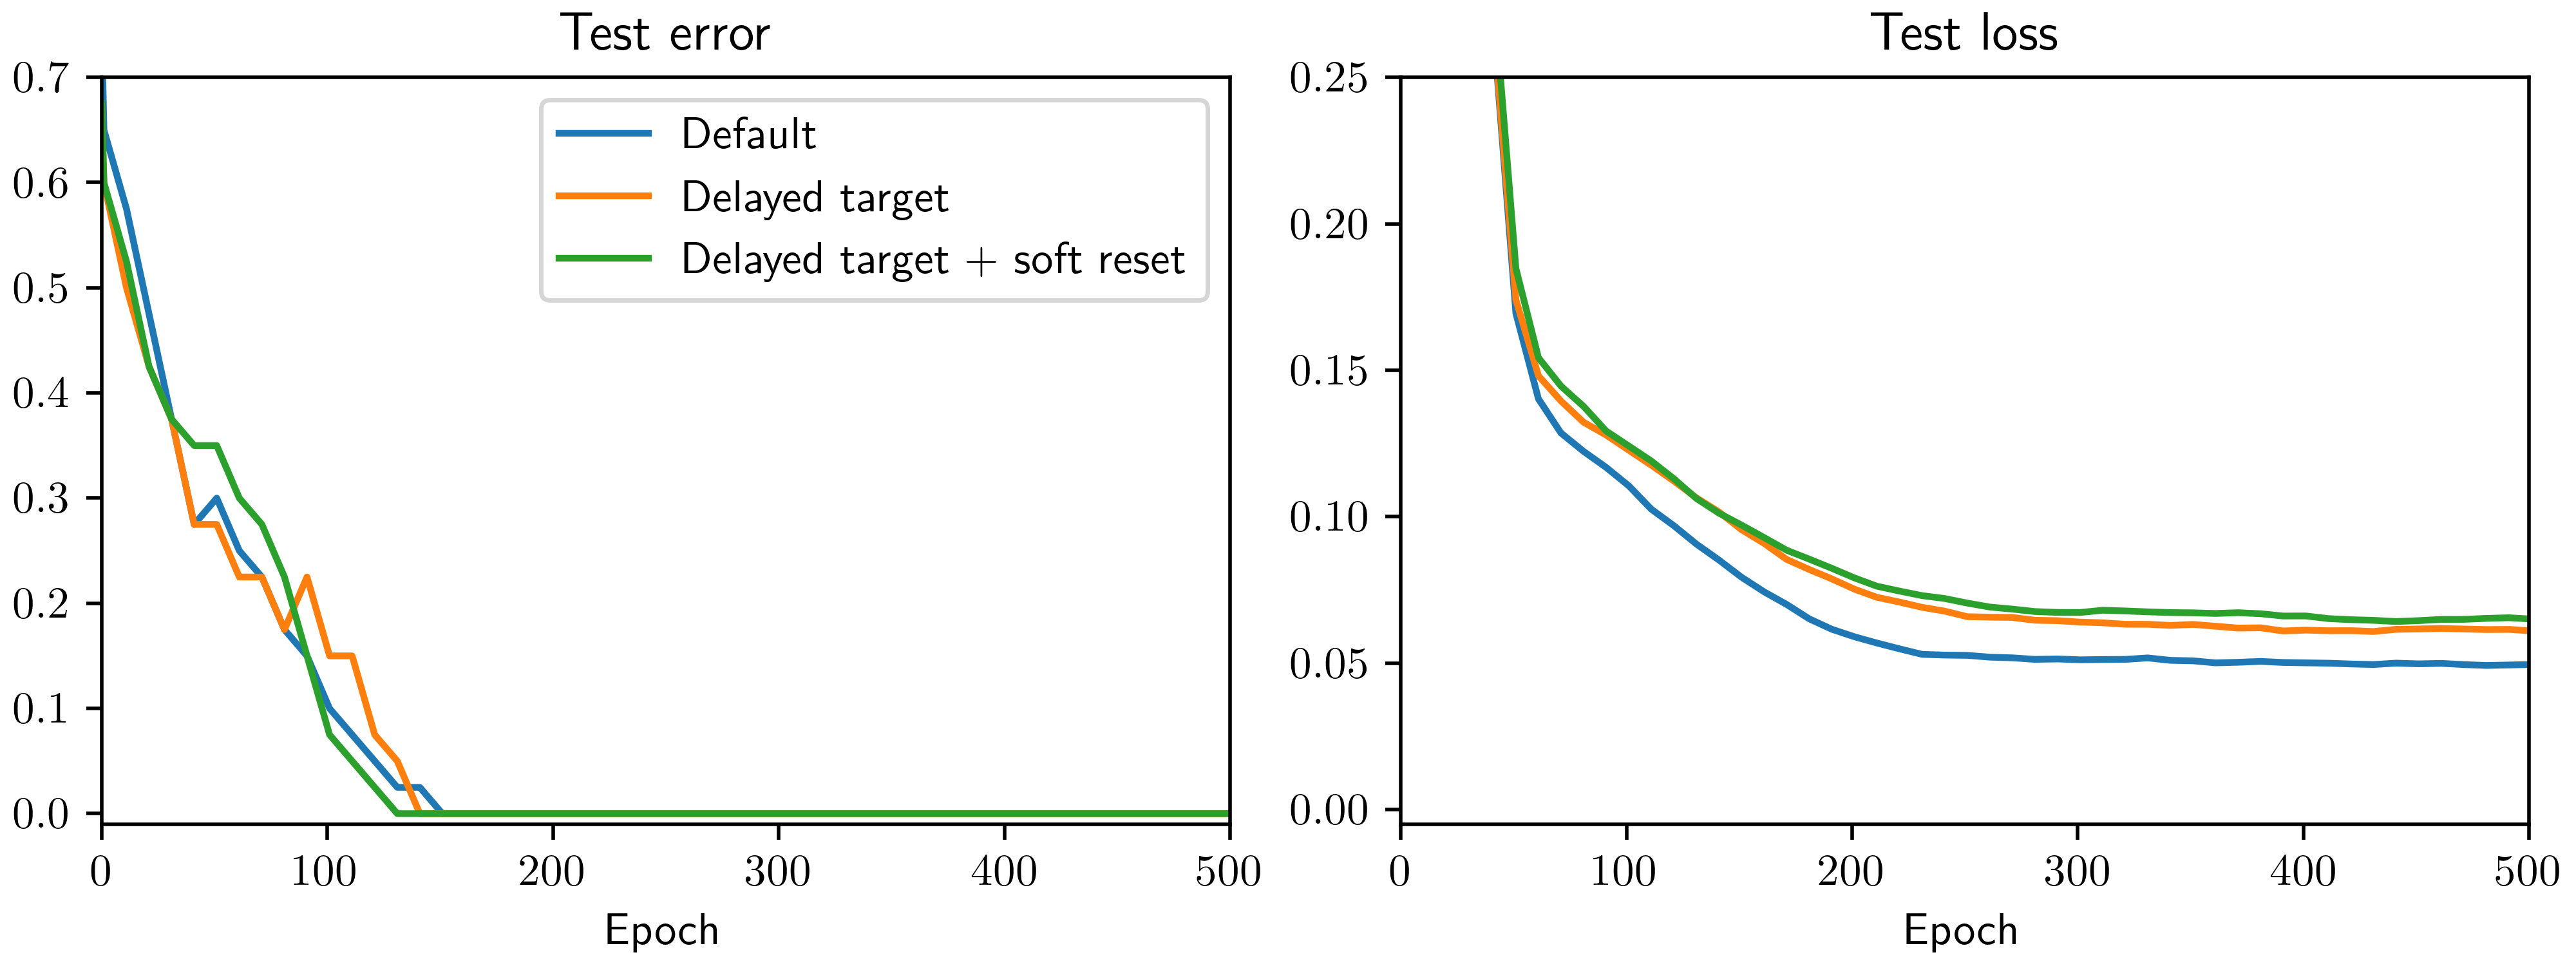
\includegraphics[width=0.9\textwidth]{fig_idle_time}
    \caption[Comparison of learning under minimal external control]{Comparison of learning under minimal external
        control. \textbf{Blue:} default parametrization for the Bars dataset. \textbf{Orange:} during the first $5ms$ of
        a training pattern, no target is provided. Afterwards training continues as usual for the remaining $45ms$.
        \textbf{Green:} Additionally, the network is not manually reset after each training sample, but simulated for
        another $15ms$ without stimulation. Increased loss of the delayed target paradigms might be explained by the
        shorter effective training time per stimulus.}
    \label{fig-idle-time}
\end{figure}

All paradigms lead to equally fast learning of the Bars dataset, with delayed target presentation causing a slightly
higher test loss. These results show that constraints like this have only miniscule impact on learning performance of
the dendritic error network. Thus, a cortical network of this kind can be expected to be indifferent to idle time in
which it is only driven by white noise. Likewise, incoming sensory information in the self-predicting state does not
cause plasticity which would drive weights away from what was previously learned. Only when a target is presented to the
output layer will weights adapt. This insight shows that the network requires even less external control, which might be
of use for improving its efficiency \todo{ref outlook}. More importantly, with the need to manually reset membrane
potentials, another biologically implausible mechanism can be omitted from simulations of this network.

It should be noted that this experiment makes the assumption that the brain is either capable of retaining an input
sequence until feedback is available, or otherwise 'replay' the pattern at a later point. While such mechanisms are much
less elegant than trace-based solutions for delayed reward signalling \citep{bellec2020solution}, the brain has been
found capable of such replays \citep{Marblestone2016}.